%% Chapter 4 — Docker and the Container Runtime Stack
\setcounter{chapter}{3}
\chapter{Docker and the Container Runtime Stack}
\chaptersubtitle{From five moves to an industry — images, registries, the OCI split, and how a GPU gets into the box}

\begin{calloutbox}{tbbblue}{tbbbluefill}
{\normalsize\bfseries\color{tbbblue}Learning objectives}\par\vspace{3pt}
\begin{tbbitemize}
  \item Explain, from the "works on my machine" handoff and the 1956 shipping-container story, why the industry adopted images: the environment becomes the artifact — and inventory precisely what is (and is not) inside one.
  \item Trace one \code{docker run} through the whole stack — CLI → dockerd → containerd → shim → runc — name each component's single job, and explain why containers survive a daemon restart (Chapter 3's shim teaser, closed).
  \item Explain the three OCI specifications (image, distribution, runtime) as the seams that make builders, registries, and runtimes swappable — including how Kata and gVisor slot in, and why the kubelet never talks to Docker.
  \item Read an image as a content-addressed artifact — manifest, config, layers, digests versus tags — and state what content-addressing buys (dedup, cache trust, tamper-evidence).
  \item Engineer a serving Dockerfile: layer ordering by rate of change, multi-stage builds, exec-form CMD (PID 1), non-root USER — and price the difference between a naive and an engineered image in pull time and gigabytes.
  \item Operate registries deliberately: layer-deduplicated push/pull, digest pinning, auth, rate limits, and the pull-storm failure mode at deploy time.
  \item Explain how a GPU actually enters a container — host driver, injected userspace, image CUDA, the toolkit hook, the device plugin — and why cgroups gate device \textit{access} but can never schedule GPU \textit{compute}.
\end{tbbitemize}
\end{calloutbox}

\vspace{5.0pt}

\begin{calloutbox}{tbbteal}{tbbtealfill}
{\normalsize\bfseries\color{tbbteal}Key terms}\par\vspace{3pt}
dependency hell · "works on my machine" · userland · break-bulk vs. the intermodal container · docker CLI · dockerd · containerd · containerd-shim · runc · OCI (image-spec / distribution-spec / runtime-spec) · config.json · CRI · dockershim (removed) · image manifest · image config · layer · digest (sha256) · tag · content-addressing · Dockerfile · build cache · .dockerignore · multi-stage build · -slim / -runtime / -devel bases · exec-form CMD · USER · registry · push / pull · pull-through cache · imagePullSecrets · rate limit · pull storm · buildx / multi-arch · NVIDIA Container Toolkit · driver / CUDA runtime split · NVIDIA\_VISIBLE\_DEVICES · device plugin · docker inspect · OOMKilled · exec format error
\end{calloutbox}

\vspace{5.0pt}

\begin{calloutbox}{tbblightgray}{tbbboxfill}
{\normalsize\bfseries\color{tbbink}Chapter outline}\par\vspace{3pt}
\textbf{4.1} From five moves to an industry    \textbf{4.2} The stack: Docker → containerd → runc, and the OCI seams    \textbf{4.3} Images as engineering: layers, digests, and the Dockerfile    \textbf{4.4} Registries: content-addressed distribution    \textbf{4.5} How a GPU gets into the box    \textbf{4.6} Reading a container like a coroner: the inspect field guide    \textbf{4.7} Lab: containerize the model server, push it, verify it — followed by a summary, exercises, and further reading.
\end{calloutbox}

\vspace{3.0pt}

\begin{calloutbox}{tbbamber}{tbbamberfill}
{\normalsize\bfseries\color{tbbamberdark}How to read this chapter}\par\vspace{3pt}
Terminal-first again: everything through §4.4 reproduces on any Docker-equipped machine (your Chapter 2 VM or a laptop; the lab's registry is a local \code{registry:2} container, so no accounts and no bill). The GPU transcripts of §4.5 are shown against a GPU node and marked as such — teams without hardware read along and reproduce them in the Week 5 managed-cluster appendix. Reproduce Transcript 4-1 before the lecture if you can: the process tree is the chapter's thesis in one screenshot.
\end{calloutbox}

\section{From Five Moves to an Industry}

Chapter 3 ended with a boast: you built a container with your bare hands. Before this chapter industrializes the trick, it owes you something more basic — an honest answer to \textit{why anyone bothers}. Not "containers are lighter than VMs" (Chapter 2 settled that), and not yet "Kubernetes needs them" (Chapter 5's business), but the original, human-sized reason: a small catastrophe so universal that every engineering team on earth has lived some version of it. Here it is, dramatized from a thousand true stories.

\subsection*{Exhibit A: the handoff}

\begin{terminalbox}
\begin{Verbatim}[breaklines=true,breakanywhere=true,fontsize=\small,formatcom=\color{tbbtermfg},codes=\tbbcodeactive]
[mon 09:12] jun   model server done! just clone the repo and run:
                  pip install -r requirements.txt && python serve.py
[mon 09:58] mina  ModuleNotFoundError: No module named 'sentencepiece'
[mon 10:20] jun   ah, install that too (added to requirements... i think)
[mon 11:03] mina  OSError: libgomp.so.1: cannot open shared object file
[mon 11:30] jun   right - sudo apt install libgomp1. which OS are you on?
[mon 13:44] mina  RuntimeError: CUDA error: no kernel image is available
                  for execution on the device
[mon 14:02] jun   hm. works on my machine :/
[tue 16:55] mina  finally running locally! deploying to the prod VM now
[tue 17:40] mina  prod python is 3.8. we built on 3.11. rolling back.
\end{Verbatim}
\end{terminalbox}
\figcaption{Exhibit 4-A  The handoff. Every line is a different layer of the same disease: the environment lived on Jun's laptop, not in the repository.}

Perform the autopsy line by line, because each failure lives at a different depth. \code{sentencepiece} — a \textbf{Python-level} dependency that never made it into requirements.txt (the file records what Jun \textit{remembered}, not what the code \textit{needs}). \code{libgomp.so.1} — a \textbf{system library} underneath pip's entire universe: no requirements.txt, however diligent, can express it, and a virtualenv fences only the Python layer, nowhere below. The CUDA error — a \textbf{userland/driver} mismatch three layers down. And Tuesday's finale — the \textbf{interpreter itself} differed between laptop and prod. The pattern: \code{requirements.txt} shipped perhaps five percent of the real environment; the rest was \textbf{state} — accumulated on one laptop over months of \code{pip install} and \code{apt install} that nobody recorded, impossible to diff, and decaying in a wiki labeled "onboarding." The disease has a name — \textbf{dependency hell} — and a catchphrase — \textbf{"works on my machine"} — and the catchphrase is precise: the machine itself had become the artifact. Pre-container treatments all dodged that fact: wikis decay, hero engineers do not scale, and full VM snapshots \textit{do} freeze the machine but as a 10 GB opaque blob nobody can diff, rebuild from source, or ship through CI.

\subsection*{Exhibit B: a box that made the world small}

The fix came from an older industry, and the lineage is worth two minutes because it explains Docker's design better than any manual. Before 1956, sea cargo moved as \textbf{break-bulk}: gangs of longshoremen hand-stowing barrels, bales, and crates, ship by ship; a vessel could spend longer in port than at sea, and loading famously cost about \textbf{\$5.86 per ton}. On April 26, 1956, a trucking magnate named \textbf{Malcom McLean} sent a converted tanker, the \textit{Ideal-X}, from Newark to Houston carrying fifty-eight identical steel boxes. Loading cost: about \textbf{\$0.16 per ton} — a \textasciitilde{}37× collapse. The genius was never the box itself; it was the \textbf{standardized corner castings}: any crane, any ship, any truck, any train could grip any container \textit{without knowing or caring what was inside}. Ports stopped opening boxes and simply moved them; handling became uniform, therefore automatable; world trade reorganized around the box within two decades. (Marc Levinson's history of this, \textit{The Box}, is this week's fun read — see Further Reading.)

Docker's founding metaphor is not decoration — the logo is literally a whale stacked with containers — and the mapping is nearly mechanical. The \textbf{image} is the box: sealed, standard shape, arbitrary contents. The \textbf{OCI specifications} (§4.2) are the corner castings: standard grips. \textbf{Runtimes and orchestrators} — runc, containerd, Kubernetes — are the cranes, ships, and trains: they handle every box identically, which is why one scheduler can run every team's workload. \textbf{Registries} (§4.4) are the ports and depots. Even the economics rhyme: the win was never that a steel box is cheap, but that \textit{handling} became uniform — and in software, "the infrastructure never opens the box" is precisely the ignorance that Chapters 5 and 6 kept calling "the platform." Your cluster does not know whether an image holds Python, Rust, or a 13 GB model server. That is a feature, and it is the entire feature.

\subsection*{So what, exactly, is in the box?}

Enough metaphor — open one. The lab's base image will do:

\begin{terminalbox}
\begin{Verbatim}[breaklines=true,breakanywhere=true,fontsize=\small,formatcom=\color{tbbtermfg},codes=\tbbcodeactive]
$ docker export $(docker create python:3.11-slim) | tar -t | wc -l
28414                    # ~28,000 files (representative count)
$ docker export $(docker create python:3.11-slim) | tar -t \
    | grep -m4 -E "libc.so|ca-certificates.crt|Seoul|bin/python3.11$"
lib/x86_64-linux-gnu/libc.so.6            # glibc: the userland floor
etc/ssl/certs/ca-certificates.crt         # trust store: HTTPS works
usr/share/zoneinfo/Asia/Seoul             # timezones. all of them.
usr/local/bin/python3.11                  # the interpreter itself
$ docker export $(docker create python:3.11-slim) | tar -t \
    | grep -cE "^boot/vmlinuz|^lib/modules"
0                        # and NO kernel. none. (Ch. 3 explained why)
\end{Verbatim}
\end{terminalbox}
\figcaption{Exhibit 4-B  Inside python:3.11-slim: a complete Linux userland — interpreter, glibc, certificates, timezone data — and, pointedly, no kernel anywhere.}

There is the honest inventory: an image is \textbf{your process's entire userland, frozen} — every file it could ever \code{open()}, from the interpreter and every site-package down through the C libraries to glibc itself, plus the quiet civilization a process assumes exists: CA certificates (why HTTPS works in a container), the timezone database, \code{/\allowbreak etc/\allowbreak passwd}, a shell. \textit{That} is what makes Mina's Monday impossible to reproduce: there is no "install X first," because every X rode along, byte-exact. Equally instructive is the anti-inventory — what is \textbf{not} in the box. \textbf{No kernel}: run \code{uname -r} inside any container and it prints the \textit{host's} kernel version, because Chapter 3's whole argument is that containers share it (this is also the crisp answer to "isn't an image just a small VM?" — a VM image must boot; a container image cannot even try). \textbf{No GPU driver} — that is host property, injected at start (§4.5). \textbf{No model weights} — model-store property, fetched at boot (Chapter 6). \textbf{No init system, no sshd, no cron} — it is one process's world, not a machine. And the definition survives even the degenerate case:

\begin{terminalbox}
\begin{Verbatim}[breaklines=true,breakanywhere=true,fontsize=\small,formatcom=\color{tbbtermfg},codes=\tbbcodeactive]
$ cat Dockerfile.scratch
FROM scratch             # the empty image: zero bytes, zero files
COPY hello /hello        # one static binary, 1.2 MB
CMD ["/hello"]
$ docker build -q -t tiny -f Dockerfile.scratch . && \
    docker export $(docker create tiny) | tar -t
hello                    # the ENTIRE filesystem. one file.
\end{Verbatim}
\end{terminalbox}
\figcaption{Exhibit 4-C  Proof by construction: an image contains exactly what you put in it. A "base image" is not an OS running underneath — it is somebody else's first few layers, adopted as your floor.}

Hold the resulting mental model — \textbf{image = frozen userland + a note on how to start it} (the "note" is §4.3's config: env, command, user) — and the handoff story ends properly: Jun's Friday afternoon becomes \code{docker build}, the box carries the whole environment including the interpreter, Mina runs it Monday 09:13 on any machine with a container runtime, and prod runs \textit{the same digest}. The wiki is retired. The machine is no longer the artifact; the artifact is the artifact.

\subsection*{From one cured laptop to an industry}

That cure, applied once, is a convenience; this chapter is about what it took to apply it \textbf{a billion times a day, on machines that have never met, assembled by no one} — and that gap is not a bigger shell script. It decomposes into three industrial problems, each mapping onto a piece of the shipping story: \textbf{packaging} (a filesystem-plus-config as a portable, verifiable artifact — the box itself, §4.3), \textbf{distribution} (moving multi-gigabyte boxes between machines in seconds — the ports, §4.4), and \textbf{lifecycle} (starting, supervising, restarting thousands, unattended — the cranes, §4.2). Docker's historical achievement was solving all three with one coherent toolset; its \textit{lasting} achievement — the reason this chapter outlives any one tool — is that the solutions were then standardized into interfaces anybody can implement (§4.2).

This chapter also completes a debt ledger that Chapters 3, 5, and 6 have been writing entries into. Chapter 3 met a mysterious shim process (PID 41288) parenting your container and promised an explanation; §4.2 pays it. Chapter 3 proved a \code{RUN rm} cannot shrink an image and gestured at "layer discipline"; §4.3 turns that into an engineering practice with a price tag. Chapter 3's cold-start arithmetic put image pulls at 25–60 seconds; §4.4 shows the machinery that makes most pulls take two. And Chapter 3's loudest negative result — \textit{no cgroup controller for GPUs} — becomes §4.5's central question: if the kernel cannot referee the GPU, how does a container get one at all, and what exactly is being promised when it does?

\subsection*{The map, before the territory}

Because this chapter names a lot of moving parts, fix the map first. When you type \code{docker run}, four programs cooperate: a \textbf{CLI} that is nothing but a REST client (the same demystification as Chapter 5's kubectl — this course keeps catching "platforms" being HTTP clients), a \textbf{daemon} (\code{dockerd}) that owns the developer-facing API and conveniences, a \textbf{lifecycle engine} (\code{containerd}) that manages images and running tasks — and which Kubernetes uses \textit{directly}, skipping Docker entirely — and a \textbf{runtime} (\code{runc}) whose entire job is Chapter 3's five moves, executed rigorously from a JSON spec, after which it \textit{exits}. Between containerd and your process stands the small, long-lived \textbf{shim} that owns it afterwards. Section 4.2 walks this chain with transcripts; the one-sentence summary to hold: \textbf{nothing in the Docker stack runs your model — the kernel does; everything else is bookkeeping around namespaces, cgroups, and overlayfs, which is exactly why every piece of it is replaceable.}

Two artifacts flow through that machinery, and they anchor the chapter's middle sections. The \textbf{image} (§4.3) is Chapter 3's overlayfs layer stack given a portable, content-addressed file format — plus a config that tells the runtime what to do with it. The \textbf{registry} (§4.4) is the distribution system those artifacts move through — a conversation conducted entirely in digests, which is why pushing a one-line code change moves kilobytes while the first pull of a CUDA base moves gigabytes. If Chapter 6's model store felt familiar when you built it — immutable versioned artifacts, checksums, "new version = new prefix" — that is because you had already been \textit{using} this chapter's registry discipline for weeks: images were the first artifact this course shipped through a content-addressed store. (In course order, of course, the rhyme runs the other way: learn it here once, recognize it everywhere.)

\subsection*{Why serving engineers care — beyond "it's the next layer down"}

\begin{tbbitemize}
  \item \textbf{The image is your deploy unit for the rest of the course.} The FastAPI server containerized in this week's lab is, byte for byte, the artifact Chapter 5 schedules (\code{registry.example.com/\allowbreak team/\allowbreak model-server}), Chapter 6 wires to the model store, and Weeks 9–14 serve, autoscale, and monitor. Every property you give it now — size, layer order, PID-1 correctness, architecture — is a property every later week inherits.
  \item \textbf{Image size is a latency and a bill.} Chapter 3 priced a 6 GB pull at 25–60 s of cold start; §4.3's worked example shows the same server shipping at a third of the size with better layer ordering — which Week 12 will convert directly into autoscaling responsiveness.
  \item \textbf{The GPU section is load-bearing for everything after.} Chapters 2, 3, and 5 each touched "GPUs are special" from their own angle (vendor sharing mechanisms; no cgroup controller; integer scheduling). §4.5 is where the three angles meet mechanically — after it, none of them is folklore.
  \item \textbf{Failures here look like magic until they look like rows.} \code{exec format error}, \code{toomanyrequests}, \code{CUDA driver version is insufficient} — §4.6's field guide files them next to Chapter 3's exit 137 and Chapter 5's Pending: signatures, causes, first commands.
\end{tbbitemize}

\begin{calloutbox}{tbbpurple}{tbbpurplefill}
{\normalsize\bfseries\color{tbbpurple}Think About It}\par\vspace{3pt}
\begin{tbbitemize}
  \item Rerun Exhibit 4-A's autopsy as a table: for each failure, name its layer (Python / system library / driver / interpreter), then say which a virtualenv would have fixed, which conda would have fixed, and which need the whole userland frozen. (Exactly one row still fails even WITH Docker — find it, and say what §4.5 does about it.)
  \item Extend the shipping analogy until it breaks: what plays the role of customs inspection? The bill of lading? Refrigerated containers? Now find one place the analogy genuinely fails — a way software boxes behave that steel boxes cannot (§4.3's layer sharing is a good place to look).
  \item Your hand-built Chapter 3 container "worked once, on one machine." List concretely what breaks when you email your rootfs tarball plus a setup script to a teammate on a different distro — and which of the three industrial problems (packaging, distribution, lifecycle) each breakage belongs to.
\end{tbbitemize}
\end{calloutbox}

\section{The Stack: Docker → containerd → runc, and the OCI Seams}

Chapter 3's very first transcript left a clue in plain sight and asked you to hold it: the container process (PID 41320) was parented not by the Docker daemon you'd have guessed, but by an anonymous intermediary, PID 41288. Time to interrogate the whole family (Figure 4-1):

\begin{terminalbox}
\begin{Verbatim}[breaklines=true,breakanywhere=true,fontsize=\small,formatcom=\color{tbbtermfg},codes=\tbbcodeactive]
$ docker run -d --name demo -m 512m --cpus 1 python:3.11 sleep 9999
3f9a1c2b77e1...                      # Ch. 3, Transcript 3-1 - same run
$ ps -eo pid,ppid,cmd | grep -E "dockerd|containerd|sleep" | grep -v grep
  912      1  /usr/bin/dockerd -H fd://
  931      1  /usr/bin/containerd
41288      1  /usr/bin/containerd-shim-runc-v2 -id 3f9a1c2b77e1...
41320  41288  sleep 9999
# note what is MISSING: runc. it started the container and exited.
# and note the shim's parent: PID 1, not containerd, not dockerd.
$ pstree -p 41288
containerd-shim(41288)---sleep(41320)
\end{Verbatim}
\end{terminalbox}
\figcaption{Transcript 4-1  The family, interrogated. Your container's ancestry contains no dockerd and no runc — just a small shim (Chapter 3's PID 41288, finally explained) holding an ordinary process.}

Read the roster with each component's single job. The \textbf{docker CLI} is a REST client: \code{docker run} is a few HTTP calls to a Unix socket (\code{docker --debug} will happily show them). \textbf{dockerd} is the daemon behind that socket — the developer-facing API, \code{docker build}, network and volume conveniences. It does \textit{not} run containers; it delegates over gRPC to \textbf{containerd}, the lifecycle engine that manages images, snapshots (overlayfs stacks — Chapter 3), and running tasks. To start a task, containerd spawns a \textbf{containerd-shim} and the shim invokes \textbf{runc}, a small standalone binary that reads a JSON spec, performs Chapter 3's five moves with production rigor, starts your process — \textit{and exits}. What remains at runtime is exactly what the transcript shows: your process, one shim, and the kernel mechanisms of Chapter 3. "The container runtime" is a setup crew, not a resident hypervisor; per-container overhead is one small process, which is a large part of why Chapter 2's isolation spectrum put containers where it did.

\subsection*{The shim earns its keep — live}

Why insert a shim at all? Because \textit{somebody} must hold the container's stdio open, collect its exit code, and reap it (Chapter 3's zombie lesson, one level up) — and that somebody must not be the daemon, or every daemon upgrade would be a fleet-wide outage. The shim is deliberately tiny, boring, and long-lived so that everything above it can be none of those things:

\begin{terminalbox}
\begin{Verbatim}[breaklines=true,breakanywhere=true,fontsize=\small,formatcom=\color{tbbtermfg},codes=\tbbcodeactive]
$ docker exec demo python -c "print('serving...')" && \
    sudo systemctl restart docker           # kill the whole daemon
serving...
$ sleep 3; docker ps --format "{{.Names}}: {{.Status}}"
demo: Up 9 minutes                          # never blinked
$ ps -o pid,ppid,cmd -p 41320
  PID   PPID  CMD
41320  41288  sleep 9999                    # same PID, same shim
# the daemon died and returned; the container never noticed.
# upgrades, crashes, restarts of dockerd/containerd: non-events.
\end{Verbatim}
\end{terminalbox}
\figcaption{Transcript 4-2  The shim's reason for existing, demonstrated: restart the entire Docker daemon and the container keeps serving under the same shim. Chapter 3's teaser, closed.}

\subsection*{The OCI seams: three specs, three swap points}

The stack's components stay honest with each other through the \textbf{Open Container Initiative} specifications — the 2015 standardization (seeded by Docker donating runc) that turned one company's product into an industry's interfaces. Three specs, one per industrial problem from §4.1. The \textbf{image-spec} defines what an image \textit{is} — manifest, config, layers, all content-addressed (§4.3's subject). The \textbf{distribution-spec} defines how images \textit{move} — the push/pull HTTP API every registry implements (§4.4's subject). And the \textbf{runtime-spec} defines how a container \textit{starts}: a bundle of rootfs + \code{config.json}, where the JSON reads like Chapter 3 translated into configuration:

\begin{terminalbox}
\begin{Verbatim}[breaklines=true,breakanywhere=true,fontsize=\small,formatcom=\color{tbbtermfg},codes=\tbbcodeactive]
$ runc spec && python3 -c "import json;c=json.load(open('config.json'));\
print(json.dumps({k:c[k] for k in ['process','root','linux']}, indent=1)[:600])"
{
 "process": { "args": ["sh"], "user": {"uid": 0}, ... },
 "root":    { "path": "rootfs", "readonly": true },
 "linux": {
  "namespaces": [ {"type":"pid"}, {"type":"network"}, {"type":"ipc"},
                  {"type":"uts"}, {"type":"mount"} ],
  "resources": { "memory": {"limit": ...}, "cpu": {...} },
  ...
# read it aloud: which namespaces to unshare (sec. 3.2), which cgroup
# values to write (sec. 3.3), which rootfs to pivot into (sec. 3.5).
\end{Verbatim}
\end{terminalbox}
\figcaption{Transcript 4-3  The OCI runtime spec's config.json is Chapter 3 as data: namespaces, cgroup resources, a root filesystem. runc is an interpreter for this file; so are Kata and gVisor.}

Standardized seams are where substitution happens, and two seams matter for this course (Figure 4-2). At the \textbf{runtime seam}, anything that accepts a runtime-spec bundle can replace runc: \textbf{Kata Containers} starts a microVM instead (a hardware boundary — Chapter 2's spectrum, unchanged callers above), \textbf{gVisor's runsc} interposes its user-space kernel (a syscall boundary). This is precisely how Chapter 2's "stronger isolation, same workflow" options plug into real clusters: one line of runtime configuration, zero changes to images or manifests. At the \textbf{orchestrator seam}, Kubernetes' kubelet speaks \textbf{CRI} — a gRPC interface — directly to containerd (the chain Chapter 5's Figure 5-2 drew): Docker's daemon was never a cluster component, and when Kubernetes removed its dockershim adapter in 2022, the industry's images kept working without modification, \textit{because images are OCI artifacts, not Docker artifacts}. That anticlimax is the whole argument for standards, and worth one italicized sentence: \textbf{Docker's lasting contribution is not the daemon; it is the specifications everyone else now implements.}

\begin{tbbfigure}
  \adjustbox{max width=0.94\linewidth,max totalheight=0.46\textheight}{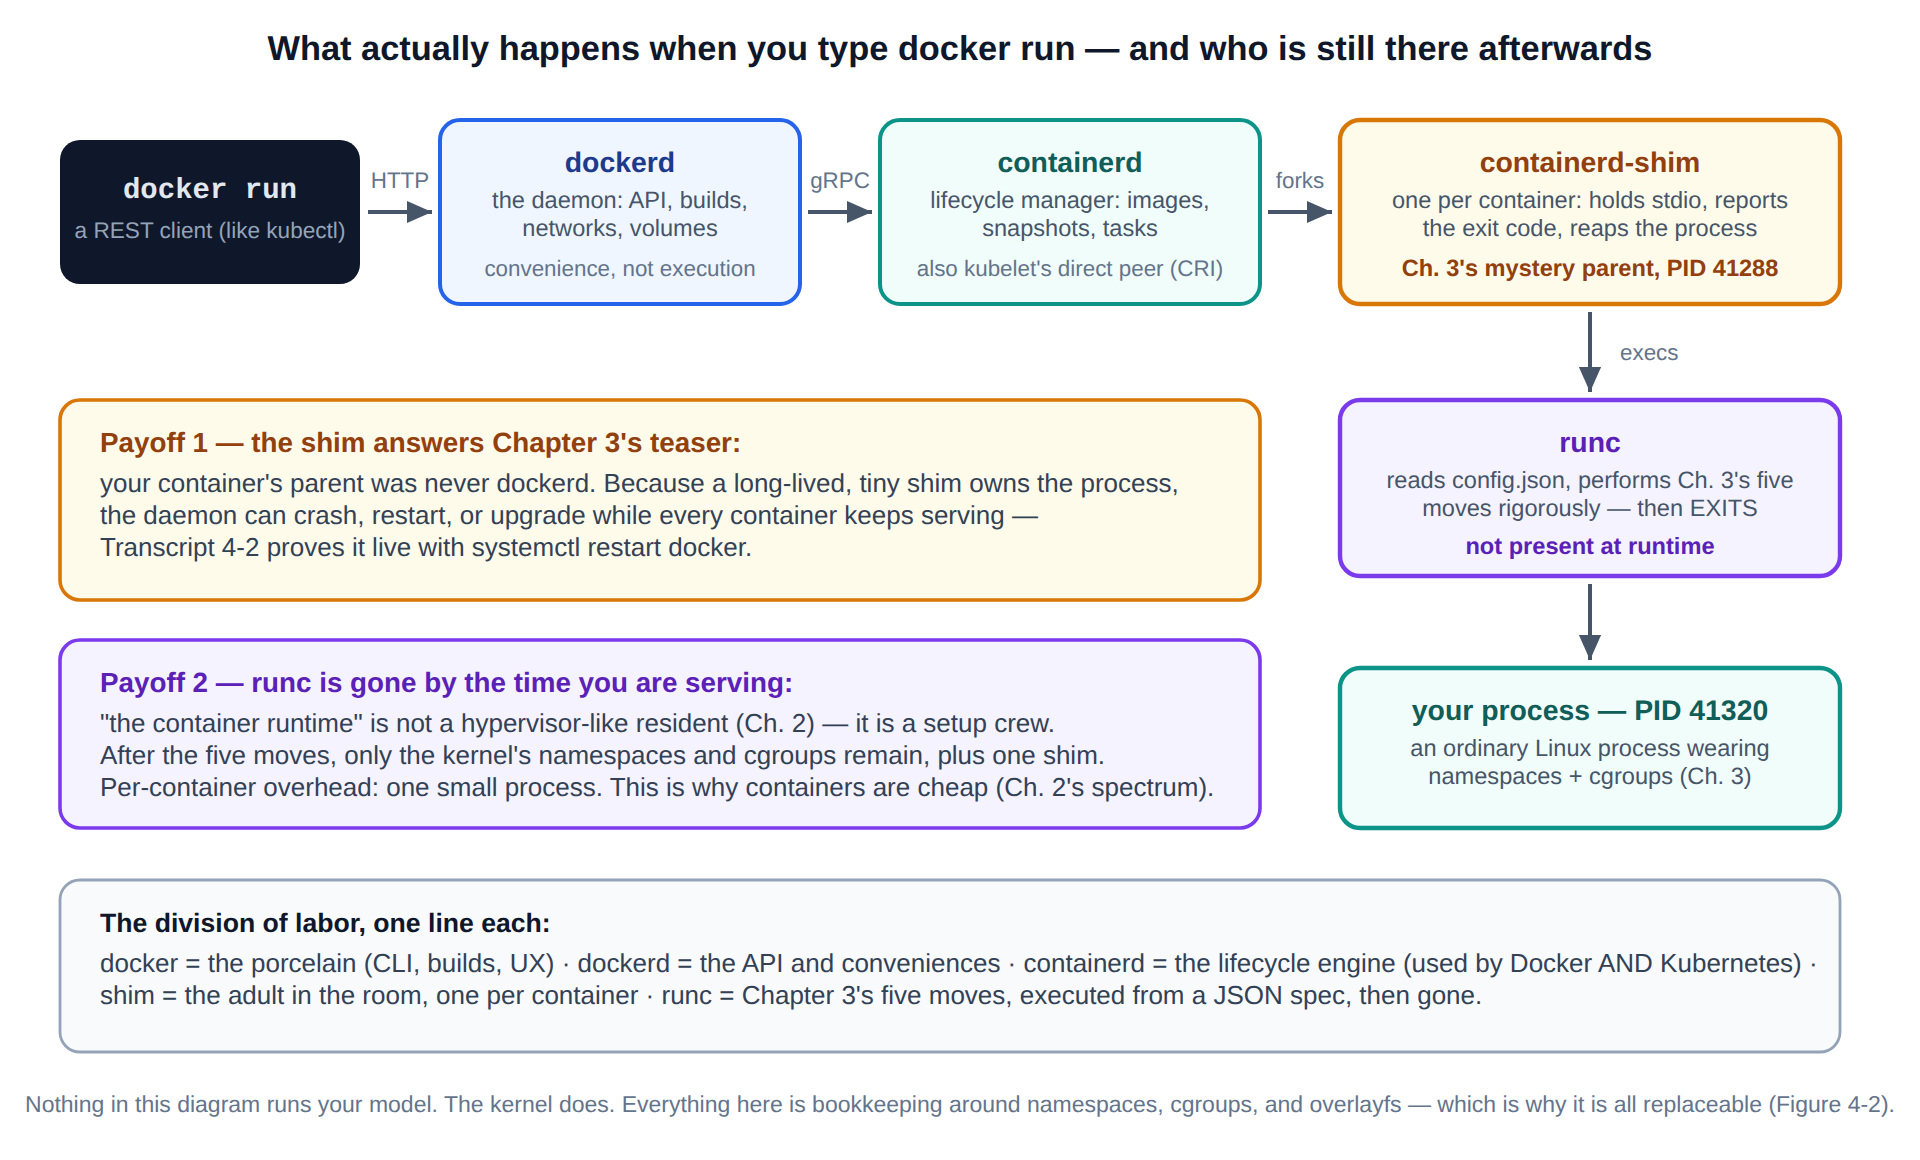
\includegraphics{figures/fig4-1_flow.png}}\\[3pt]
  \figcaption{Figure 4-1  The docker run flow, and who remains afterwards: the CLI and daemons are bookkeeping; runc performs Chapter 3's five moves and exits; one shim per container holds what must be held.}
\end{tbbfigure}

\begin{tbbfigure}
  \adjustbox{max width=0.94\linewidth,max totalheight=0.46\textheight}{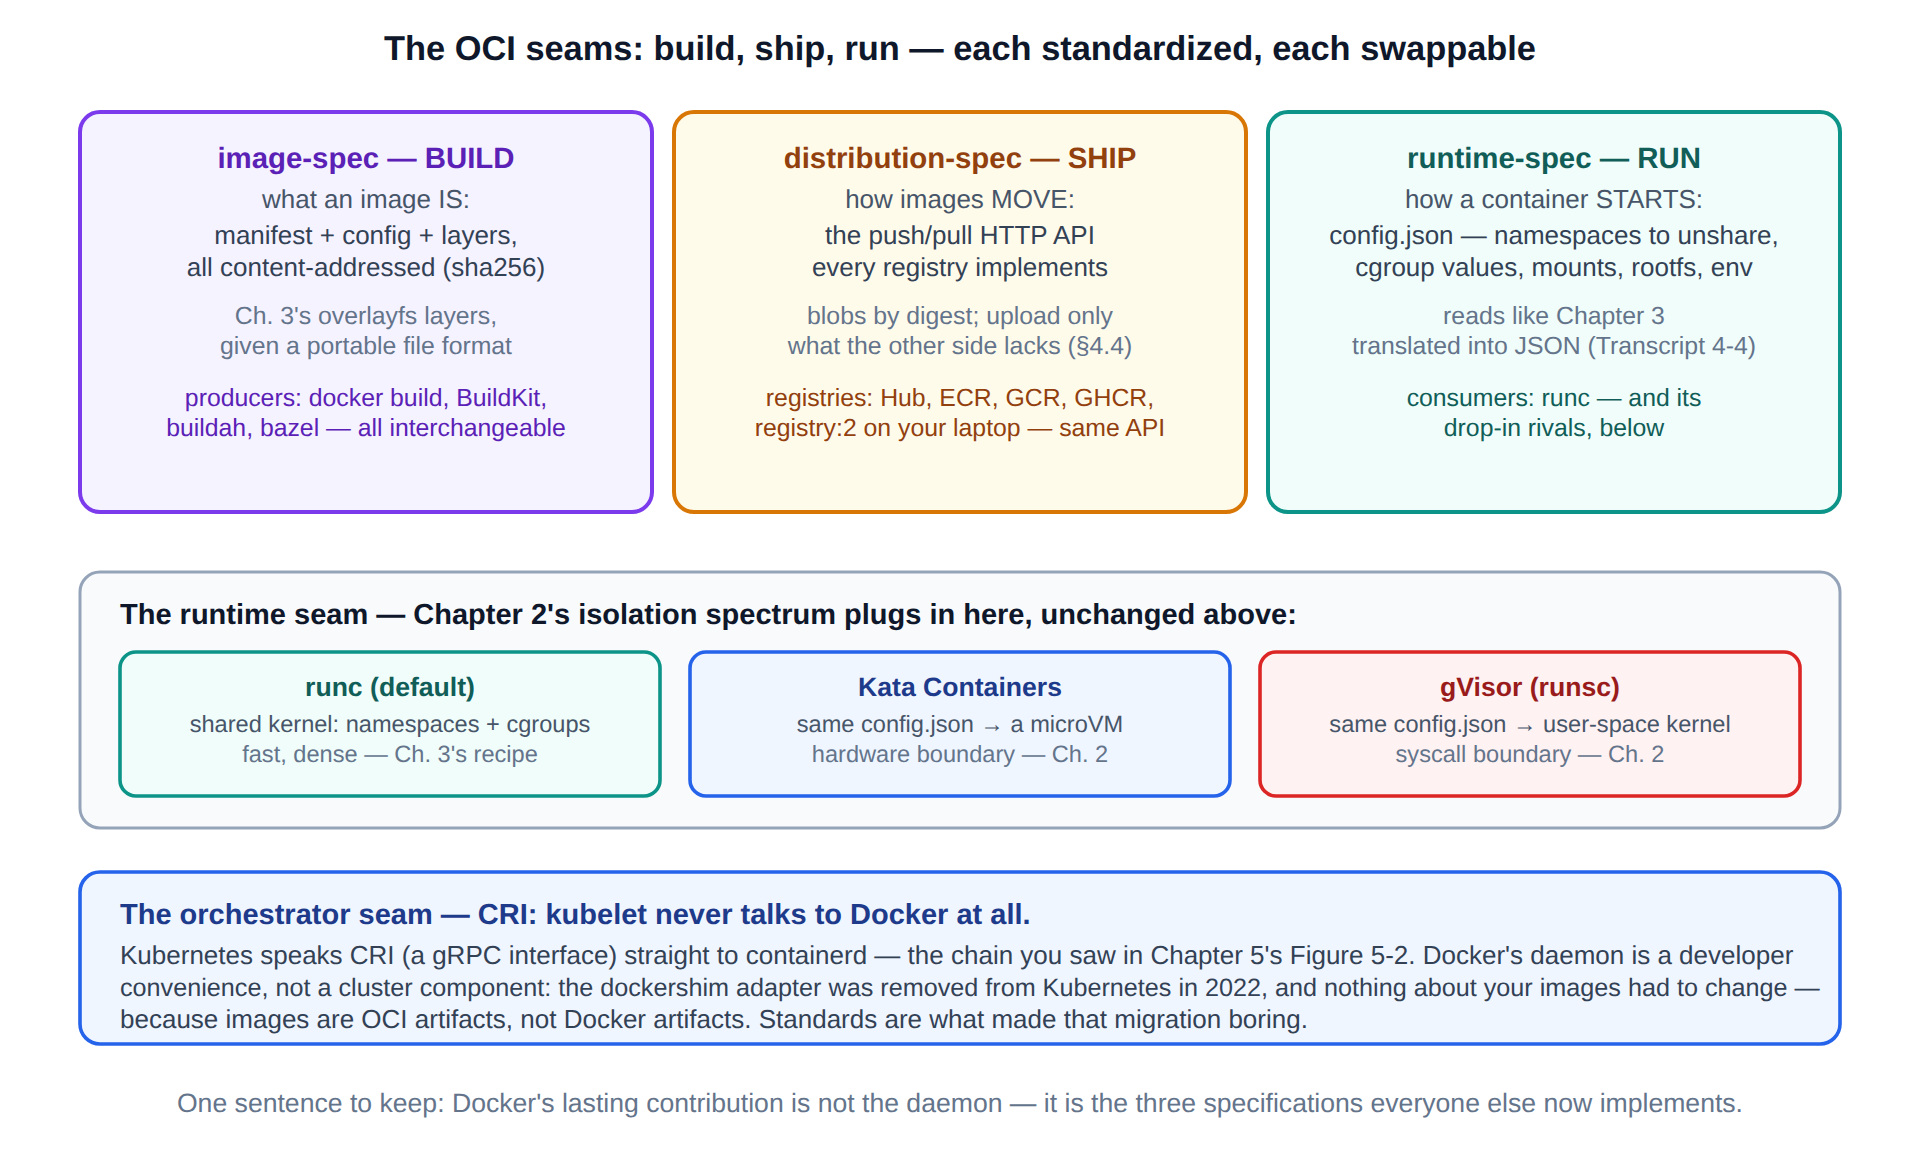
\includegraphics{figures/fig4-2_oci.png}}\\[3pt]
  \figcaption{Figure 4-2  The OCI seams. Build, ship, and run are separate specs — so builders, registries, and runtimes are independently swappable, and the kubelet needs no Docker at all.}
\end{tbbfigure}

\begin{calloutbox}{tbbpurple}{tbbpurplefill}
{\normalsize\bfseries\color{tbbpurple}Think About It}\par\vspace{3pt}
\begin{tbbitemize}
  \item Rank the stack's components (dockerd, containerd, shim, runc) by how bad their crash is for a serving fleet — justify each rank with what state or duty the component holds. (The answer explains why the architecture puts the smallest program closest to your process.)
  \item Kata substitutes a microVM at the runtime seam "with zero changes above." Using Chapters 2 and 3, name two things that DO silently change for the workload (think: kernel identity, /proc contents, device access) — the seam standardizes the contract, not the physics.
  \item The dockershim removal broke almost nothing — but it did break \textit{something} for some teams. Guess what kind of workflow depended on the Docker daemon being on every node (hint: docker build inside CI pods, docker.sock mounts), and what the OCI-native replacements are.
\end{tbbitemize}
\end{calloutbox}

\section{Images as Engineering: Layers, Digests, and the Dockerfile}

Chapter 3 taught the mechanism (overlayfs: reads fall through, writes copy up, deletes leave whiteouts) and its economics (dedup, cache, cold-start pulls). This section turns mechanism into \textbf{artifact}: what precisely is the thing you push, how is it named, and how do you author one that behaves well in production? Start by taking a real image apart (Figure 4-3):

\begin{terminalbox}
\begin{Verbatim}[breaklines=true,breakanywhere=true,fontsize=\small,formatcom=\color{tbbtermfg},codes=\tbbcodeactive]
$ docker build -t model-server:v1 . && docker images model-server
REPOSITORY     TAG   IMAGE ID       SIZE
model-server   v1    9f2c4a01be77   2.4GB
$ docker image inspect model-server:v1 --format \
    '{{.Architecture}} {{len .RootFS.Layers}} layers'
amd64 9 layers
$ docker history model-server:v1 --format "{{.Size}}\t{{.CreatedBy}}" | head -5
40kB    COPY serve.py /app/serve.py
1.9GB   RUN pip install -r requirements.txt
0B      WORKDIR /app
120MB   FROM python:3.11-slim
# every Dockerfile step that touched the filesystem = one layer,
# stackable and shippable exactly as Chapter 3 described.
\end{Verbatim}
\end{terminalbox}
\figcaption{Transcript 4-4  An image disassembled: layers map one-to-one onto filesystem-touching Dockerfile steps, and the artifact's identity is a digest, not the friendly name you typed.}

Structurally, an OCI image is three kinds of object, each named by the sha256 of its bytes. The \textbf{manifest} is the tiny root document: it lists the digests of one \textbf{config} and N \textbf{layers}. The config carries the runtime half — env, \code{Cmd}, \code{User}, exposed ports: the things runc will be told — plus the ordered layer list. The layers are Chapter 3's read-only overlayfs strata as compressed tarballs. \textbf{Content-addressing} is the load-bearing choice: because every object's name \textit{is} its hash, identical layers are stored and transferred once no matter how many images share them (dedup), a machine that has \code{sha256:22...} cached can trust it absolutely without asking who built it (cache trust — this is why layer caching works across machines that never met, the question Chapter 3 posed), and any tampering changes the name (integrity). A \textbf{tag} like \code{:v7}, by contrast, is a \textit{mutable pointer} into this immutable world — a nickname someone can move. The operational rule falls straight out: humans speak tags; \textbf{deploys pin digests} (\code{image@sha256:aa41f9...}) or use registry-enforced immutable tags. Chapter 6 asked you to run the same discipline for model versions; here is where the course learned it.

\begin{tbbfigure}
  \adjustbox{max width=0.94\linewidth,max totalheight=0.46\textheight}{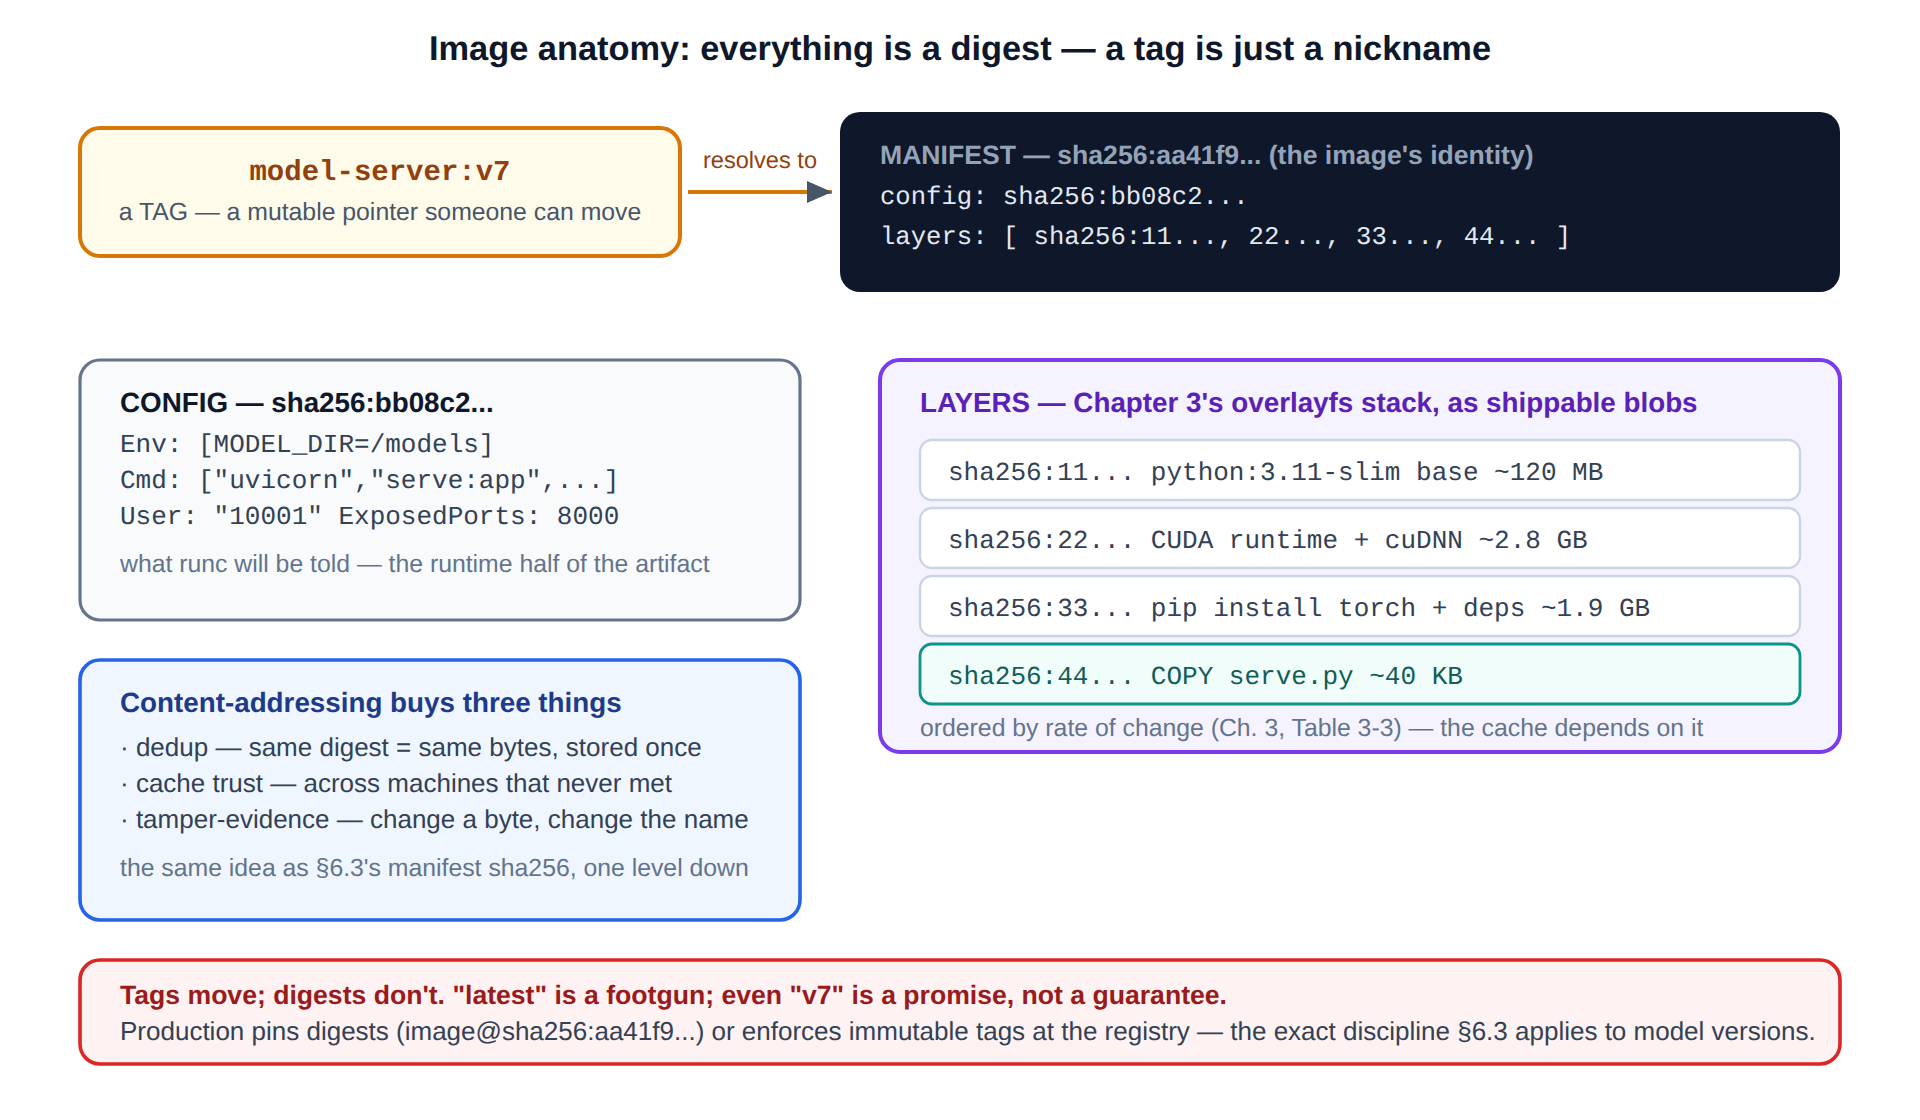
\includegraphics{figures/fig4-3_image.png}}\\[3pt]
  \figcaption{Figure 4-3  Image anatomy: a manifest naming a config and layers, everything content-addressed. Tags are mutable nicknames; digests are identity — production deploys pin the latter.}
\end{tbbfigure}

\subsection*{The Dockerfile, engineered line by line}

Authoring the image is where this course's accumulated lessons become one file. The Dockerfile below is the course model server's, and every line is a callback with a receipt (Figure 4-4 annotates it in full):

\begin{terminalbox}
\begin{Verbatim}[breaklines=true,breakanywhere=true,fontsize=\small,formatcom=\color{tbbtermfg},codes=\tbbcodeactive]
# ---- stage 1: builder - compilers live here, and die here ----
FROM python:3.11 AS builder
COPY requirements.txt .
RUN pip install --prefix=/venv -r requirements.txt

# ---- stage 2: runtime - what actually ships ----
FROM python:3.11-slim
COPY --from=builder /venv /venv         # deps: change monthly
ENV PATH=/venv/bin:$PATH
RUN useradd -u 10001 serve
USER 10001                              # non-root (Ch. 3)
COPY serve.py /app/serve.py             # code: changes DAILY - last!
EXPOSE 8000
CMD ["uvicorn", "serve:app", "--host", "0.0.0.0", "--port", "8000"]
#   ^^ EXEC form: the server IS PID 1; SIGTERM lands (Ch. 3's bug)
\end{Verbatim}
\end{terminalbox}
\figcaption{Transcript 4-5  The course Dockerfile. Ordering implements Chapter 3's cache economics; multi-stage separates build-time from runtime dependencies; the last line permanently fixes Chapter 3's CMD-form bug.}

Three decisions carry most of the value. \textbf{Ordering by rate of change} is Chapter 3's Table 3-3 made executable: base and dependencies (slow-changing) sit low, \code{serve.py} (daily-changing) sits last, so the daily rebuild reuses every layer but a 40 KB one — and, per §4.4, the daily \textit{push and pull} move kilobytes too. One corollary deserves its own sentence: \code{COPY requirements.txt} + \code{pip install} come \textit{before} any \code{COPY . .} — copy the whole tree first and every code edit invalidates the dependency layer, the classic inversion Chapter 3 priced at twenty minutes a rebuild. (The companion tool is \textbf{.dockerignore}: build context that never enters the image cannot invalidate caches — exclude \code{.git}, datasets, and, per Chapter 6, any local model weights.) \textbf{Multi-stage builds} resolve a genuine tension: installing scientific Python needs compilers and headers (\textasciitilde{}1.9 GB of them), but \textit{running} it needs none — so stage 1 installs into \code{/\allowbreak venv} with the full toolchain and stage 2 copies only \code{/\allowbreak venv} onto a slim base. Build-time dependencies stop being runtime payload; the CPU lab image drops from 2.4 GB to \textasciitilde{}610 MB. \textbf{PID-1 correctness and non-root}: the exec-form \code{CMD} makes your server PID 1 so SIGTERM actually lands (Chapter 3's rollout tape; Chapter 5's draining; Chapter 6's 502 alignment — one line, three chapters of payoff), and \code{USER 10001} means an application compromise lands as an unprivileged user (Chapter 3's escape-consequence lesson, applied at build time).

\begin{tbbfigure}
  \adjustbox{max width=0.94\linewidth,max totalheight=0.46\textheight}{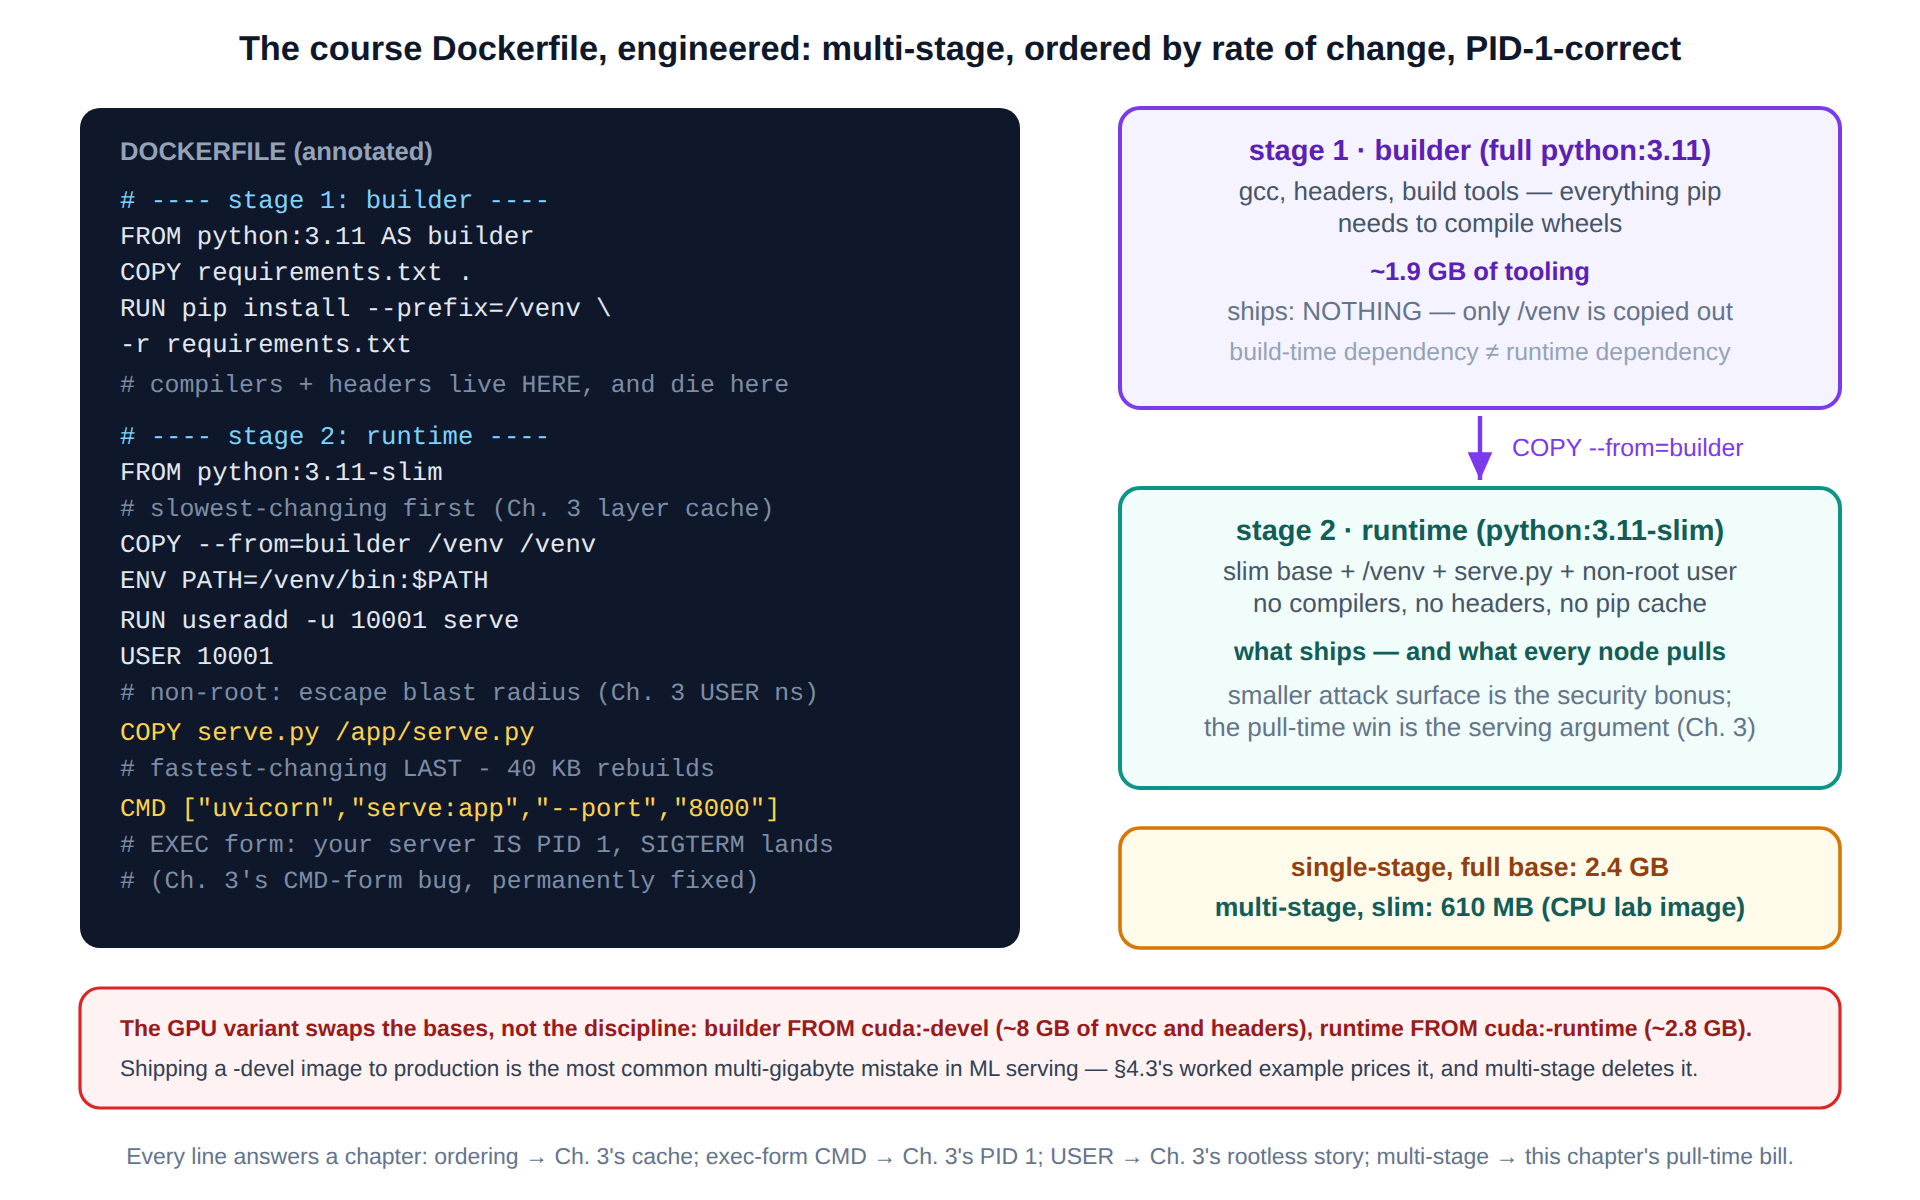
\includegraphics{figures/fig4-4_dockerfile.png}}\\[3pt]
  \figcaption{Figure 4-4  The Dockerfile engineered: multi-stage separates the 1.9 GB toolchain from the 610 MB artifact; ordering protects the cache; the CMD and USER lines are Chapter 3's lessons, frozen into the build.}
\end{tbbfigure}

\subsection*{The GPU flavor: the CUDA tag zoo, priced}

GPU serving images inherit the same discipline with one loaded decision: \textbf{which CUDA base}. NVIDIA publishes three flavors per CUDA version — \code{base} (driver-facing libraries only), \code{runtime} (adds the CUDA runtime and libraries like cuDNN: what \textit{running} frameworks need), and \code{devel} (adds nvcc, headers, static libs: what \textit{compiling} needs, at \textasciitilde{}8 GB). The recurring multi-gigabyte mistake is shipping \code{devel} to production because "it worked in dev." The multi-stage pattern makes the right thing mechanical — build custom kernels in a \code{devel} builder stage, ship a \code{runtime} final stage — and the worked example prices the difference:

\begin{calloutbox}{tbbamber}{tbbamberfill}
{\normalsize\bfseries\color{tbbamberdark}Worked example — the image diet, in pull time and dollars}\par\vspace{3pt}
The GPU serving image, three ways (representative sizes; pulls at Chapter 3's effective 100–250 MB/s):

\begin{tbbitemize}
  \item \textbf{Naive:} single-stage on cuda:-devel, COPY-before-pip inversion — \textbf{9.8 GB}. Fresh-node pull: 40–100 s; and \textit{every code deploy} re-ships the 4 GB dependency layer because the inversion invalidates it.
  \item \textbf{Ordered:} same base, layers ordered correctly — still 9.8 GB on first pull, but code deploys now move \textasciitilde{}40 KB. Half the problem solved by moving two lines.
  \item \textbf{Engineered:} multi-stage onto cuda:-runtime — \textbf{3.1 GB}. Fresh-node pull: 12–31 s. Cold-start line item (Wk 12) cut by \textasciitilde{}3×; node disk \textasciitilde{}7 GB lighter per image version; registry storage and egress down in proportion.
\end{tbbitemize}

At fleet scale the arithmetic compounds: 20 fresh nodes × (9.8 − 3.1) GB = \textbf{134 GB less registry traffic per full-fleet cold pull}, and every autoscale-up gets the \textasciitilde{}3× faster bar. Same server, same model, same hardware — the difference is one Dockerfile.
\end{calloutbox}

\vspace{3.0pt}

One boundary note completes the section, because it decides \textit{what goes in the artifact at all}. The image carries the CUDA \textbf{userland} (runtime, cuDNN) but never the \textbf{driver} — that is the host's, injected at start (§4.5's subject). And per Chapters 3 and 6, it carries \textbf{no model weights} — those live in the model store, loaded at boot. What remains is exactly what an image should be: code, dependencies, and configuration — the parts that change on the code cadence and deserve the code's review process.

\begin{calloutbox}{tbbpurple}{tbbpurplefill}
{\normalsize\bfseries\color{tbbpurple}Think About It}\par\vspace{3pt}
\begin{tbbitemize}
  \item A teammate's "quick fix" adds COPY . /app as the third line of the Dockerfile "so everything is available." Trace the consequences through build time, push size, node pulls, and Week 12's autoscaler — then fix it with two moved lines and a .dockerignore.
  \item Why does the exec-form CMD line pay off in three different chapters (3, 5, 6)? Name the mechanism in each: what specifically breaks with shell form at a rollout, at a drain, at the load balancer?
  \item Multi-stage builds separate build-time from runtime dependencies. Give the model-serving analogue one level up: what does §6.3's model store separate, and why is "the training container serves traffic" the same mistake as "ship the devel image"?
\end{tbbitemize}
\end{calloutbox}

\section{Registries: Content-Addressed Distribution}

A registry is a deceptively simple thing: an HTTP service implementing the OCI distribution-spec, storing blobs (layers, configs, manifests) by digest and serving them back. Docker Hub, ECR, GCR, GHCR, and the \code{registry:2} container you will run in the lab expose the \textit{same API} — which is why \code{docker push} and a kubelet's image pull work identically against any of them, and why the blobs themselves conventionally live on object storage (a fact Chapter 6 will give a whole contract to). The interesting engineering is not the storage; it is the \textbf{conversation} — because push and pull are the same negotiation in opposite directions: \textit{"here is a manifest; which of its digests do you not have?"} Only missing blobs ever move. Dedup is not an optimization; it is the protocol (Figure 4-5):

\begin{terminalbox}
\begin{Verbatim}[breaklines=true,breakanywhere=true,fontsize=\small,formatcom=\color{tbbtermfg},codes=\tbbcodeactive]
$ docker tag model-server:v1 localhost:5000/team/model-server:v1
$ docker push localhost:5000/team/model-server:v1
a1b2c3d4e5f6: Pushed        # 120MB  base (first push: everything moves)
b2c3d4e5f6a1: Pushed        # 1.9GB  deps
c3d4e5f6a1b2: Pushed        # 40kB   serve.py
v1: digest: sha256:aa41f9... size: 2415
# now change one line of serve.py, rebuild as :v2, push again:
$ docker build -q -t localhost:5000/team/model-server:v2 . && \
    docker push localhost:5000/team/model-server:v2
a1b2c3d4e5f6: Layer already exists
b2c3d4e5f6a1: Layer already exists
f6a1b2c3d4e5: Pushed        # 40kB - the only bytes that moved
v2: digest: sha256:bc52a0... size: 2415
\end{Verbatim}
\end{terminalbox}
\figcaption{Transcript 4-6  The protocol at work: the second push moves 40 KB, because every other digest "already exists." The pull side is symmetric — which is what makes daily deploys cheap and cold nodes expensive.}

The pull side completes the economics. A node keeps a \textbf{local layer cache} (containerd's snapshots); pulling \code{v2} onto a node that served \code{v1} fetches one 40 KB layer, which is why Chapter 5's rolling updates are quiet events on warm fleets. The expensive case is the \textbf{fresh node} — everything must come down once, at Chapter 3's 25–60 s for CUDA-sized images — and the pathological case is the \textbf{pull storm}: a scale-out or full-fleet deploy hitting many fresh nodes at once, multiplying gigabytes by node count through one registry path, precisely when you are most impatient (Week 12 meets this as the autoscaling cold-start tax; mitigations, in escalating order: the §4.3 diet, node image caches and pre-pulling, a pull-through mirror in-region, and lazy-loading snapshotters for the truly ambitious). Note also what the transcript prints at the end of every push: the \textbf{manifest digest}. That string is the deployable identity — Chapter 5's manifests should reference it (\code{image@sha256:...}) or an immutable tag, because tags drift and "it deployed \textit{something} called v2" is not an audit trail. Week 13's pipelines will promote digests between environments for exactly this reason.

\begin{tbbfigure}
  \adjustbox{max width=0.94\linewidth,max totalheight=0.46\textheight}{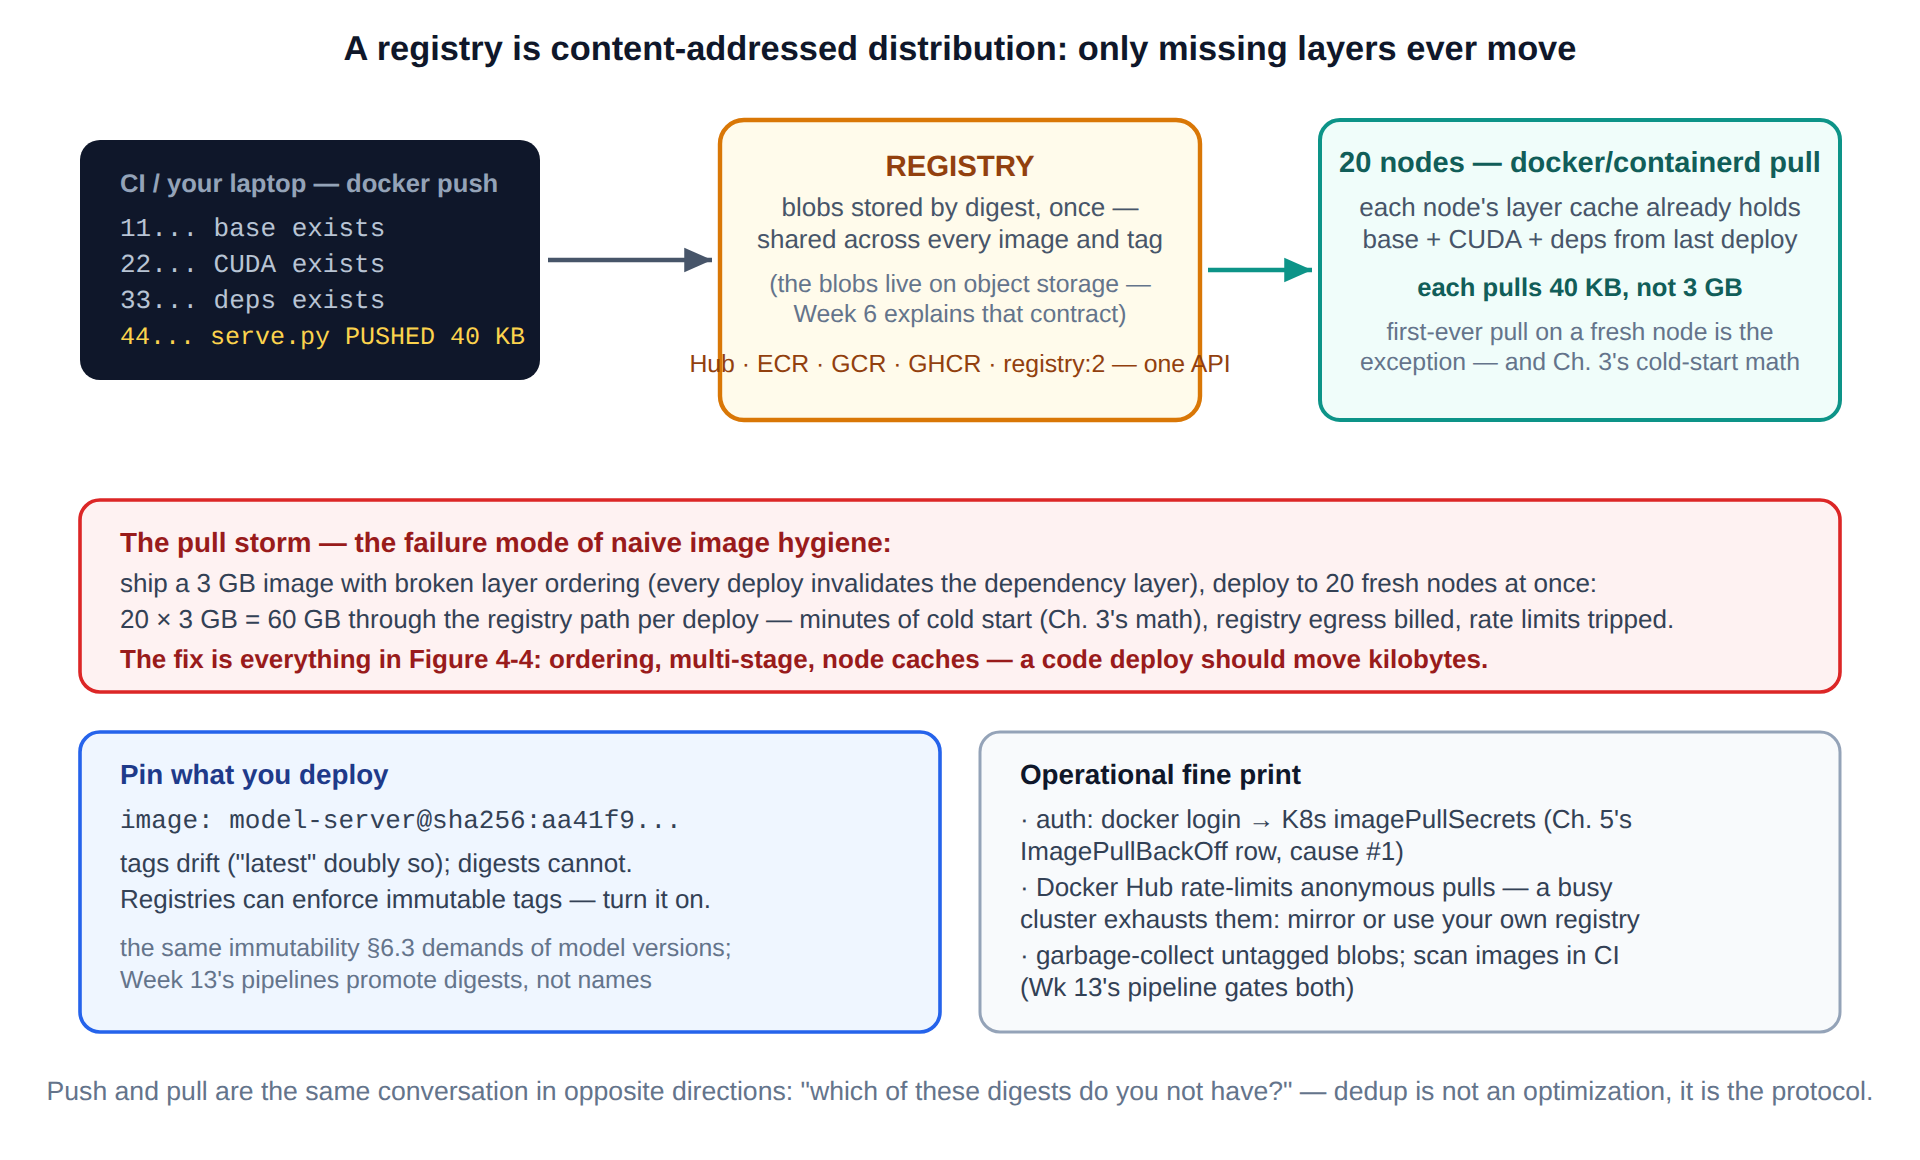
\includegraphics{figures/fig4-5_registry.png}}\\[3pt]
  \figcaption{Figure 4-5  Content-addressed distribution: pushes and pulls move only missing digests; node caches make code deploys kilobyte-sized; fresh nodes and pull storms are the expensive exceptions to engineer around.}
\end{tbbfigure}

\subsection*{Operational fine print that becomes incidents}

\begin{tbbitemize}
  \item \textbf{Authentication.} \code{docker login} stores a credential; Kubernetes needs the same material as an \code{imagePullSecrets} reference (Chapter 5's ImagePullBackOff row, cause \#1). Cloud registries integrate with instance/pod IAM — on a well-set-up cluster, nodes pull private images with no static secret at all (the Chapter 6 keyless pattern, again).
  \item \textbf{Rate limits.} Docker Hub throttles anonymous pulls aggressively enough that a modest cluster can exhaust the allowance mid-deploy — \code{toomanyrequests: You have reached your pull rate limit} is a genuine outage class (§4.6). The structural fix is not "log in harder": mirror the public bases you depend on into your own registry (a pull-through cache is one flag on \code{registry:2}), which also survives upstream outages and deletions.
  \item \textbf{Hygiene.} Tags accumulate; untagged manifests and orphaned blobs linger until garbage-collected — registries have retention policies for a reason, and "we never GC'd and the registry bill doubled" is a real quarterly surprise. Pair retention with \textbf{scanning} (CVE scans on push) — Week 13's pipeline gates on both.
  \item \textbf{Architecture.} A repository can hold a \textbf{multi-arch manifest list} — the same tag resolving to amd64 and arm64 images. Build on an Apple-silicon laptop without \code{--platform} and you will meet §4.6's \code{exec format error} the moment a cloud node pulls your arm64-only image. \code{docker buildx --platform linux/\allowbreak amd64,linux/\allowbreak arm64} publishes both; CI should own this, not laptops.
\end{tbbitemize}

\begin{calloutbox}{tbbpurple}{tbbpurplefill}
{\normalsize\bfseries\color{tbbpurple}Think About It}\par\vspace{3pt}
\begin{tbbitemize}
  \item Using Transcript 4-6's mechanics: your team deploys 6×/day to 20 warm nodes, and the image is layered correctly. Estimate daily registry traffic — then re-estimate with the COPY-inversion bug from §4.3. (This is Chapter 3's Think question, now with the distribution half priced in.)
  \item A pull-through mirror caches public images in-region. Enumerate what it protects you from (three distinct failure/cost classes) and the one new failure it introduces.
  \item Why should Week 13's pipeline promote digests rather than re-tagging images per environment ("staging" → "prod")? Give the concrete race/rollback scenarios each approach produces.
\end{tbbitemize}
\end{calloutbox}

\section{How a GPU Gets Into the Box}

Now the question this course has been saving since Chapter 2, and the syllabus's own parenthesis: \textit{why can't cgroups schedule GPU compute — and given that they can't, how does a container use a GPU at all?} Start from what a container fundamentally is (Chapter 3): namespaces and cgroups around a process, \textbf{virtualizing nothing}. A GPU therefore cannot be "emulated into" a container the way Chapter 2's virtio emulated disks into VMs; the container must be handed the real thing. And "the real thing" is a \textit{stack} with a fault line in it: a \textbf{kernel module} (\code{nvidia.ko}) and its exactly-version-matched \textbf{driver userspace libraries} on the host, and above them the \textbf{CUDA userland} — runtime, cuDNN, framework — that applications link against. The fault line dictates the packaging rule that makes ML images portable at all: \textbf{the image carries CUDA userland; the host carries the driver; nothing in the image may depend on a specific driver build} (Figure 4-6).

\begin{tbbfigure}
  \adjustbox{max width=0.94\linewidth,max totalheight=0.46\textheight}{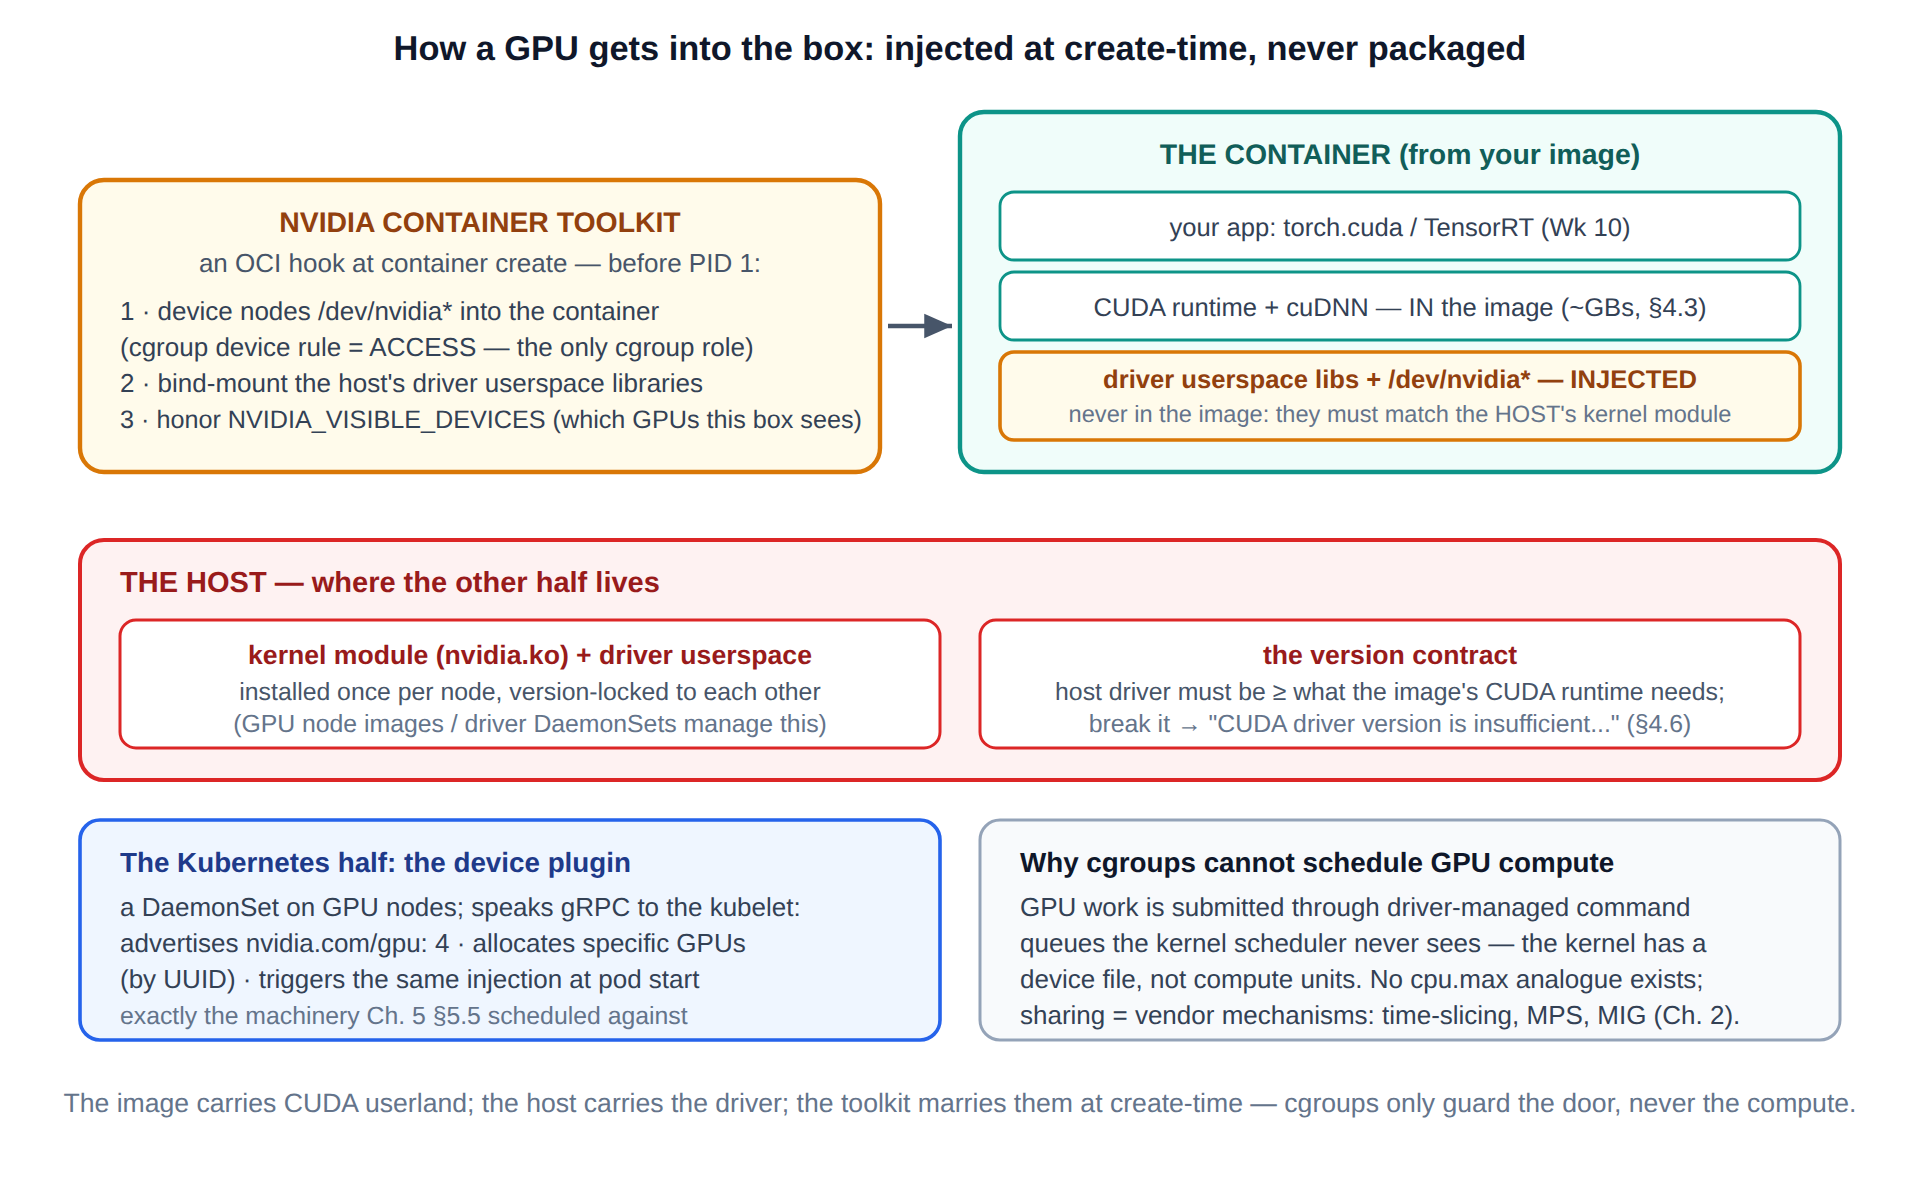
\includegraphics{figures/fig4-6_gpu.png}}\\[3pt]
  \figcaption{Figure 4-6  The GPU enters at create-time: the toolkit's OCI hook injects device nodes and the host's driver userspace into a container whose image carries only CUDA userland. cgroups guard the door; the driver owns the compute.}
\end{tbbfigure}

\subsection*{The mechanism: an OCI hook, three injections}

The \textbf{NVIDIA Container Toolkit} implements the marriage as an OCI-level hook: a shim runtime (\code{nvidia-container-runtime}) that receives the runtime-spec bundle, edits it, and hands it to plain runc. At container create — before your PID 1 exists — it performs three injections. First, the \textbf{device nodes}: \code{/\allowbreak dev/\allowbreak nvidia0}, \code{/\allowbreak dev/\allowbreak nvidiactl}, \code{/\allowbreak dev/\allowbreak nvidia-uvm} appear in the container, and a cgroup \textit{device rule} permits them — pause on that clause, because it is the \textbf{only} cgroup involvement in the entire GPU story: an allow/deny on opening a file, Chapter 3's "gate access" claim made concrete. Second, the \textbf{driver userspace libraries} are bind-mounted from the host — the halves that must match \code{nvidia.ko} come from the same machine as \code{nvidia.ko}, which is the whole trick. Third, environment (\code{NVIDIA\_VISIBLE\_DEVICES}) selects \textit{which} GPUs this container may see, which is how one 4-GPU node hands different devices to different containers:

\begin{terminalbox}
\begin{Verbatim}[breaklines=true,breakanywhere=true,fontsize=\small,formatcom=\color{tbbtermfg},codes=\tbbcodeactive]
$ docker run --rm --gpus '"device=0"' nvidia/cuda:12.4-runtime nvidia-smi \
    --query-gpu=index,name,memory.total --format=csv,noheader
0, NVIDIA A10G, 23028 MiB
$ docker inspect $(docker ps -lq) --format '{{json .HostConfig.DeviceRequests}}'
[{"Driver":"nvidia","Count":0,"DeviceIDs":["0"],"Capabilities":[["gpu"]]}]
# and the injected mounts, visible like any other config:
$ docker inspect $(docker ps -lq) | grep -c "nvidia"
23        # device nodes + driver libs + env - all inspectable
# the failure mode, staged: an image whose CUDA is newer than the host driver:
$ docker run --rm --gpus all nvidia/cuda:99.9-runtime python3 -c "..."
CUDA driver version is insufficient for CUDA runtime version
# the version contract of Figure 4-6, breached on purpose (sec. 4.6).
\end{Verbatim}
\end{terminalbox}
\figcaption{Transcript 4-7  GPU access is configuration, not magic: a device request in HostConfig, injected nodes and mounts you can inspect — and the classic error when the image's CUDA outruns the host's driver.}

\subsection*{The Kubernetes half — and the question answered properly}

On a cluster, discovery and allocation move up a level. The \textbf{device plugin} — a DaemonSet on GPU nodes — speaks gRPC to the kubelet: it advertises \code{nvidia.com/\allowbreak gpu: 4} into the node's capacity (the exact number Chapter 5's scheduler budgeted against), and when a pod requesting a GPU lands, it tells the kubelet \textit{which} physical devices (by UUID) to grant; the kubelet's CRI call then triggers the same toolkit injection you just watched Docker perform. Nothing new happens at the bottom; Kubernetes adds inventory and placement on top of an unchanged mechanism — Chapter 5 §5.5's "extended resources are integers" now has its machine room.

Which leaves the syllabus's \textit{why}. The kernel schedules what it can see: CPU time (it owns the run queues — hence \code{cpu.max} can freeze a task mid-burst) and memory (it owns the page tables — hence \code{memory.max} can refuse an allocation). GPU compute is invisible to it by construction: user processes submit work through \textbf{driver-managed command queues} — often mapped straight into user space so submission does not even syscall — and the GPU's own engines and firmware pick what runs next. To the kernel, the entire GPU is a device file it can permit or deny opening; there is no kernel-visible unit of "GPU time" for a cgroup controller to meter, so none exists. Everything downstream in this course follows from that one sentence: sharing had to come from the \textbf{vendor layer} (Chapter 2's time-slicing, MPS, MIG — the driver and hardware \textit{can} see the queues); Kubernetes, refusing to promise what nothing below can enforce, schedules GPUs as \textbf{indivisible integers} (Chapter 5); and the OOM-style safety nets you enjoyed for memory simply do not exist for VRAM — exhaust it and you get Chapter 3's \textit{other} OOM, the catchable CUDA allocator error, with the kernel nowhere in the story.

\begin{calloutbox}{tbbblue}{tbbbluefill}
{\normalsize\bfseries\color{tbbblue}The GPU story, assembled across four chapters}\par\vspace{3pt}
\begin{tbbitemize}
  \item \textbf{Ch. 2:} the hardware can be shared — but only by vendor mechanisms: PCIe passthrough, vGPU, time-slicing, MPS, MIG.
  \item \textbf{Ch. 3:} the kernel cannot referee it — no cgroup GPU controller; only device-file access control.
  \item \textbf{Ch. 4 (here):} so access is \textit{injection}: host driver + device nodes married to image CUDA userland at create-time, by an OCI hook; discovery and allocation via the device plugin.
  \item \textbf{Ch. 5:} so orchestration treats GPUs as integer extended resources — no fractions, no overcommit, requests = limits — and fractional demand routes back to Ch. 2's mechanisms (Week 12 operationalizes them).
\end{tbbitemize}
\end{calloutbox}

\vspace{3.0pt}

\begin{calloutbox}{tbbpurple}{tbbpurplefill}
{\normalsize\bfseries\color{tbbpurple}Think About It}\par\vspace{3pt}
\begin{tbbitemize}
  \item Why would baking the host's driver libraries into the image — "it worked on my node!" — be a portability time bomb? Trace what happens when the fleet's node pool upgrades its driver version under a fixed image.
  \item NVIDIA\_VISIBLE\_DEVICES is enforcement by injection: a container simply never sees devices it wasn't granted. Compare this to memory.max's enforcement model (Ch. 3). Which failure modes does each admit? (Hint: what happens if two containers are \textit{granted the same} GPU?)
  \item Using this section plus Ch. 2: a teammate proposes "let's write a cgroup controller for GPU time — how hard can it be?" Write the two-paragraph technical rejection: what would the kernel need to see that it cannot, and where would the metering have to live instead?
\end{tbbitemize}
\end{calloutbox}

\section{Reading a Container Like a Coroner: The Inspect Field Guide}

This course's field-guide habit — signatures, causes, first commands — started in Chapter 3 with one exit code and grows a level each chapter. The docker-layer edition has a single anchor tool: \textbf{docker inspect}, the platform's sworn testimony about what was \textit{actually} configured and what \textit{actually} happened, as JSON. Everything you declared (image, env, limits, devices) and everything the stack recorded (state, exit code, OOM flag, restart count) is in there — the skill is knowing which field answers which question. The lab's required exercise is the best introduction, because it closes a loop this course opened in Chapter 3's very first transcript:

\begin{terminalbox}
\begin{Verbatim}[breaklines=true,breakanywhere=true,fontsize=\small,formatcom=\color{tbbtermfg},codes=\tbbcodeactive]
$ docker run -d --name demo -m 512m --cpus 1 model-server:v1
$ docker inspect demo --format \
    'mem={{.HostConfig.Memory}} nanocpus={{.HostConfig.NanoCpus}}'
mem=536870912 nanocpus=1000000000     # your flags, recorded verbatim
$ PID=$(docker inspect demo --format '{{.State.Pid}}') && echo $PID
41320
$ CG=$(cat /proc/$PID/cgroup | cut -d: -f3) && \
    cat /sys/fs/cgroup$CG/memory.max /sys/fs/cgroup$CG/cpu.max
536870912                             # the SAME number, in the kernel
100000 100000                         # --cpus 1, in Ch. 3 grammar
# intent (inspect) == enforcement (cgroupfs): the ghostwriter, audited.
# this is Transcript 3-1 closed from both ends - and the lab's Part B.
\end{Verbatim}
\end{terminalbox}
\figcaption{Transcript 4-8  The audit the syllabus asks for: docker inspect shows the recorded intent; the cgroup filesystem shows the kernel's enforcement; the numbers match because Chapter 3's ghostwriter is this chapter's stack.}

Fix a small map of the JSON, because six fields answer ninety percent of questions. \textbf{.State} — is it running, and if not, \textit{how did it end}: \code{ExitCode}, \code{OOMKilled}, \code{Error}, timestamps (a dead container is a corpse with paperwork; \code{docker logs} still works on it — the flight-recorder habit from Chapter 5's \code{--previous}, one layer down). \textbf{.Config} — what the \textit{image} said: env, \code{Cmd}, \code{User}, exposed ports. \textbf{.HostConfig} — what the \textit{operator} said: limits, restart policy, devices, mounts, port publishes; when intent and reality disagree, this is where the intent is written. \textbf{.GraphDriver} — the overlayfs directories (Chapter 3's lower/upper/merged, with real paths you can \code{ls}). \textbf{.NetworkSettings} — IP, ports, and the veth story of §3.2. \textbf{.RootFS.Layers} — the digest list, for confirming \textit{which bytes} you are actually running when a tag has betrayed you. With the map in hand, the recurring failures file themselves (Figure 4-7):

\begin{tbbfigure}
  \adjustbox{max width=0.94\linewidth,max totalheight=0.46\textheight}{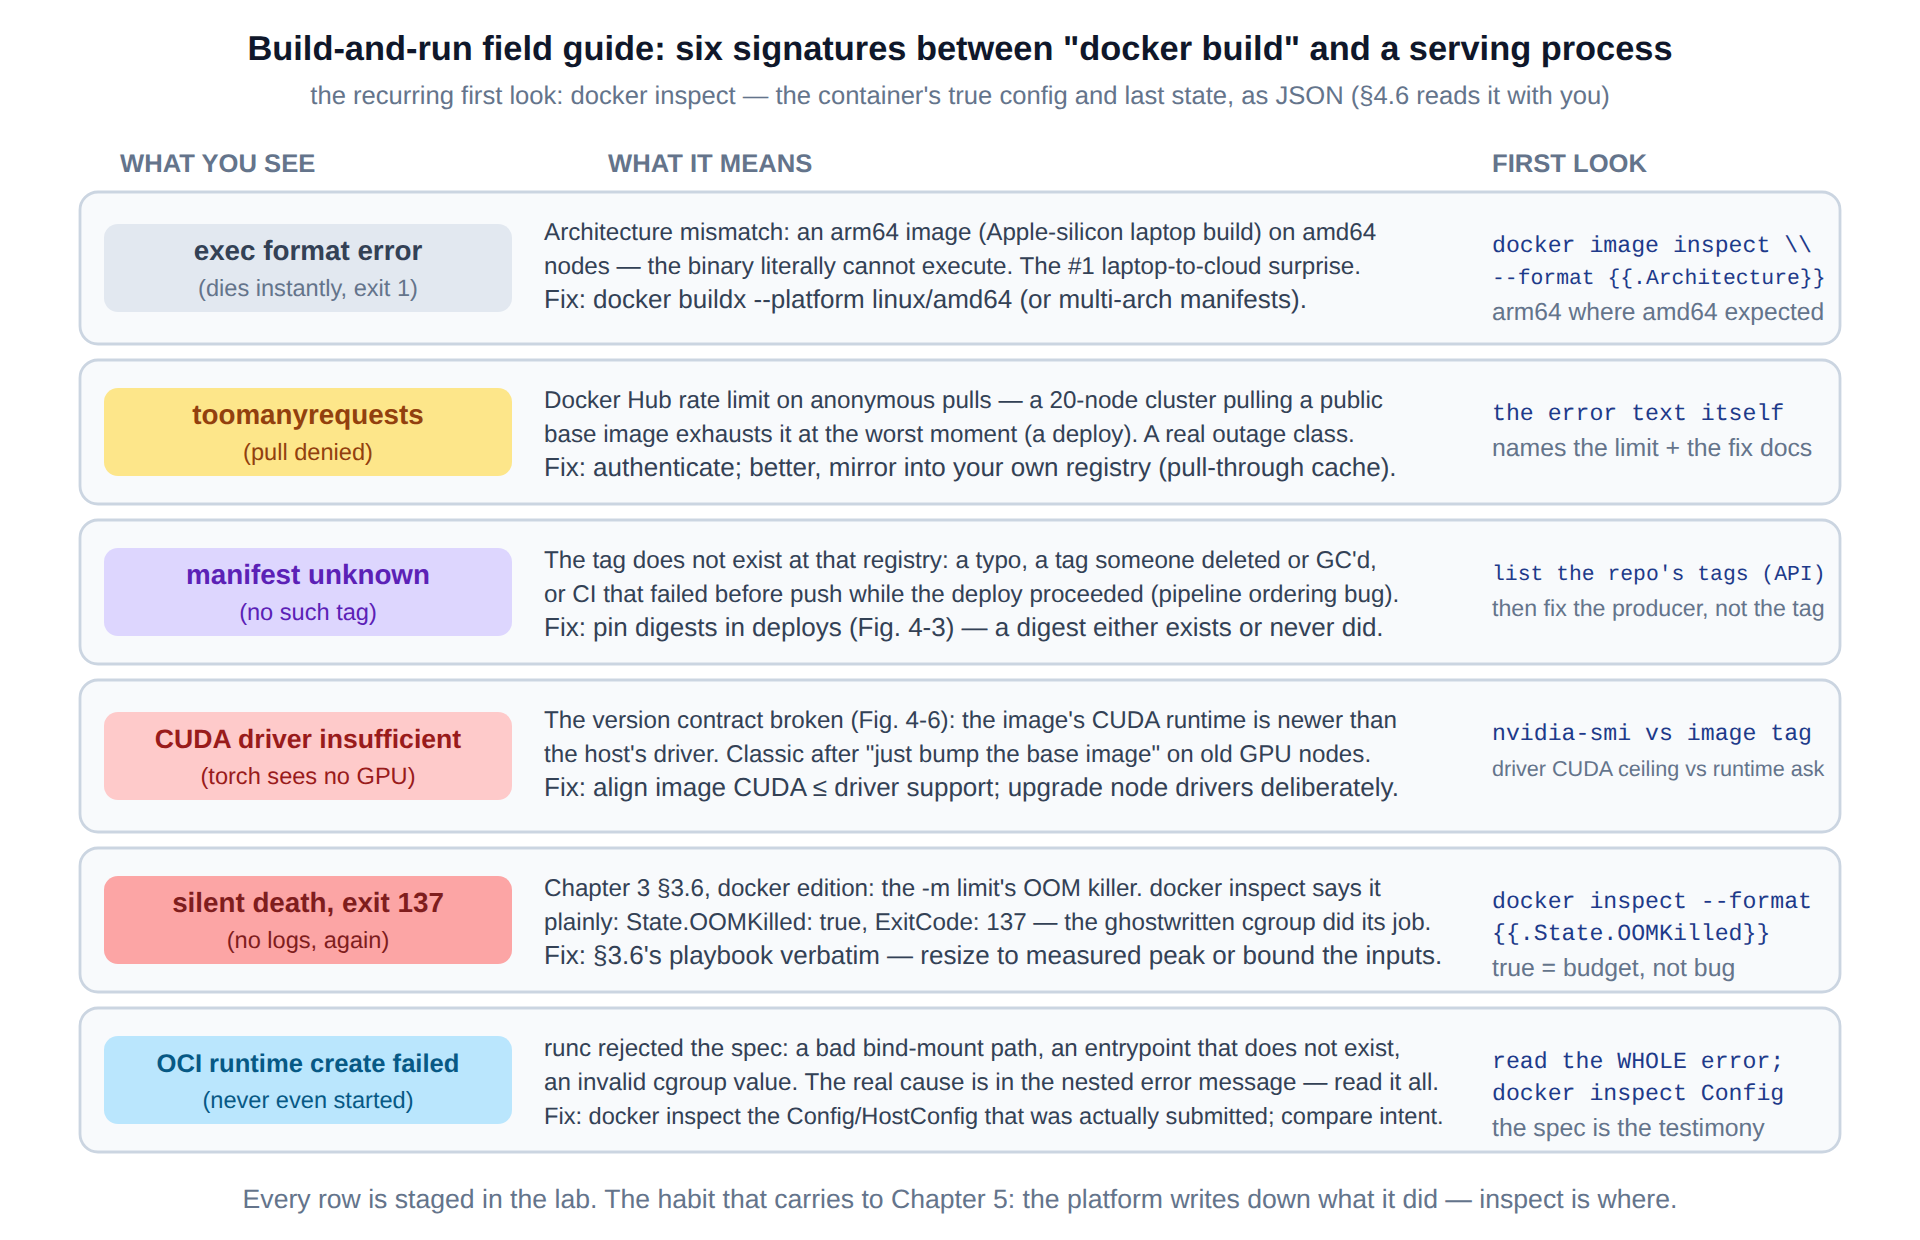
\includegraphics{figures/fig4-7_fieldguide.png}}\\[3pt]
  \figcaption{Figure 4-7  The build-and-run field guide: architecture mismatches, rate limits, vanished tags, the CUDA version contract, the docker-flavored OOM, and runc's spec rejections — each with its first command.}
\end{tbbfigure}

\begin{tbbitemize}
  \item \textbf{exec format error, instantly} — the binary cannot execute on this CPU: an arm64 image (Apple-silicon laptop default) on amd64 nodes. The \#1 laptop-to-cloud surprise since 2021. Confirm with \code{docker image inspect --format '\{\{.Architecture\}\}'}; fix in CI with \code{buildx --platform linux/\allowbreak amd64} (or publish multi-arch). File next to it: \code{no matching manifest for linux/\allowbreak amd64} — same disease, caught at pull time instead of exec time.
  \item \textbf{toomanyrequests at pull} — Docker Hub's anonymous rate limit, exhausted by your own fleet mid-deploy. Authenticate as triage; mirror the public bases you depend on as the fix (§4.4) — you do not want your deploy cadence coupled to a third party's throttle.
  \item \textbf{manifest unknown} — the tag is not there: typo, deleted/GC'd tag, or a pipeline that deployed before its build pushed. The durable fix is §4.3's: deploy digests, which either exist or never did — a digest cannot be half-pushed.
  \item \textbf{CUDA driver version is insufficient for CUDA runtime version} — Figure 4-6's version contract, breached: the image's CUDA userland is newer than the host driver, classically after "just bump the base image" lands on an older node pool. Compare \code{nvidia-smi}'s driver/CUDA ceiling on the host against the image tag; upgrade drivers deliberately, not incidentally.
  \item \textbf{Silent death, exit 137} — Chapter 3 §3.6 in docker packaging: \code{.State.OOMKilled: true} says the \code{-m} wall was enforced. The conversation is unchanged — resize to measured peak or bound inputs — and the flag is the one-command proof that it was budget, not bug.
  \item \textbf{OCI runtime create failed} — runc rejected the spec before your process existed: a bind-mount source that isn't there, an entrypoint path that doesn't exist in the image, an invalid cgroup value. The true cause is the \textit{innermost} nested error — read the whole line, then \code{docker inspect} the Config/HostConfig that was actually submitted and diff it against your intent.
\end{tbbitemize}

One habit ties the section to the rest of the course: \textbf{the platform writes down what it did.} Chapter 3 read the kernel's ledgers (\code{/\allowbreak proc}, cgroupfs, dmesg); this section reads the runtime's (\code{inspect}, \code{events}, \code{logs}); Chapter 5 read the orchestrator's (describe, events); Chapter 6 read the door's (status codes, target health). Four layers, one discipline — and an incident is just the practice of asking each layer for its testimony in the right order.

\begin{calloutbox}{tbbpurple}{tbbpurplefill}
{\normalsize\bfseries\color{tbbpurple}Think About It}\par\vspace{3pt}
\begin{tbbitemize}
  \item A container runs perfectly under docker run -it but dies instantly under Kubernetes with exit 127 ("not found"). Using the .Config/.HostConfig split, hypothesize the two most likely divergences between what you ran interactively and what the manifest submitted (hint: entrypoint overrides, env-dependent paths).
  \item Design the five-line CI gate that would have prevented every row of Figure 4-7 that is preventable pre-deploy. Which two rows fundamentally cannot be caught in CI, and what runtime check covers each instead?
  \item docker inspect shows .HostConfig.Memory = 536870912 but the container is using 800 MB happily. Before calling it a bug: list the three explanations Chapter 3 equips you to check, in the order you would check them (hint: which cgroup is actually enforcing, page cache vs anon, and who might have edited the live cgroup).
\end{tbbitemize}
\end{calloutbox}

\section{Lab: Containerize the Model Server, Push It, Verify It}

This week's lab produces the course's central artifact: the FastAPI model server as a well-engineered image, in a registry, verified down to the cgroup files — the exact image Chapter 5 deploys to Kubernetes and Chapter 6 wires to the model store. Everything runs on your Chapter 2 VM or a laptop; the registry is a local \code{registry:2} container (free, instant, same API as the real thing); the GPU part is an optional appendix for teams with hardware. Deliverable: the artifacts checklist below plus a one-page report, each observation naming its section.

\subsection*{Part A — build it well, and prove the layers behave}

Write \code{serve.py} (the handout scaffolds a FastAPI app with \code{/\allowbreak predict}, \code{/\allowbreak healthz}, and \code{/\allowbreak ready} — the same three endpoints Chapters 5 and 6 probe) and containerize it twice. First the \textbf{naive} build: single-stage, full base, \code{COPY . .} before \code{pip install}. Then the \textbf{engineered} build: Transcript 4-5's multi-stage Dockerfile with a \code{.dockerignore}. Record for each: image size (\code{docker images}), layer map (\code{docker history}), and — the measurement that makes ordering visceral — \textbf{rebuild time and "bytes that would move" after a one-line change to serve.py} (rebuild both; watch the naive build re-run pip while the engineered build reuses every cached layer and rebuilds in seconds). Confirm architecture explicitly (\code{docker image inspect --format '\{\{.Architecture\}\}'}) — Apple-silicon teams add \code{--platform linux/\allowbreak amd64} and note the emulation cost in their report.

\subsection*{Part B — run it, limit it, audit it (the syllabus's inspect exercise)}

Run the engineered image with real budgets — \code{-m 512m --cpus 1 -p 8080:8000} — and reproduce Transcript 4-8 end to end on your own container: \code{inspect} the recorded intent, walk \code{/\allowbreak proc/\allowbreak <pid>/\allowbreak cgroup} to the cgroup directory, and photograph \code{memory.max} and \code{cpu.max} agreeing with your flags. (You have now personally closed the loop Chapter 3 opened: flag → daemon → containerd → runc → kernel file.) Then two live verifications. \textbf{PID-1 correctness}: \code{docker stop} the container and time it — exec-form CMD drains and exits on SIGTERM in under a second, while a deliberately shell-form variant (the handout provides one) hangs the full 10 s grace and gets SIGKILLed; capture both timings. \textbf{The docker-flavored OOM}: rerun with \code{-m 128m}, drive the toy inference loop until the 137, and collect \code{.State.OOMKilled: true} — Chapter 3's evidence chain with this chapter's tooling.

\subsection*{Part C — a registry of your own, and the protocol observed}

Run \code{docker run -d -p 5000:5000 --name registry registry:2}, tag and push the engineered image, and read the layer-by-layer output. Then the two experiments that teach the protocol. \textbf{Dedup}: change one line of serve.py, rebuild as \code{:v2}, push, and capture the wall of \code{Layer already exists} with one small \code{Pushed} — Transcript 4-6, yours. \textbf{Digest discipline}: record each push's returned digest, pull by digest (\code{docker pull localhost:5000/\allowbreak team/\allowbreak model-server@sha256:...}), then deliberately re-tag \code{:v2} at a \textit{different} image and demonstrate that the tag now lies while the digest cannot — write the one-sentence policy this argues for (you already know it from §6.3's model store; here is where it comes from). Finally, stage two field-guide rows on purpose: pull a nonexistent tag (\code{manifest unknown}) and, if any team member has an ARM machine, run its unflagged build on x86 (\code{exec format error}) — screenshots into the report.

\begin{calloutbox}{tbbpurple}{tbbpurplefill}
{\normalsize\bfseries\color{tbbpurple}Lab checklist}\par\vspace{3pt}
\begin{tbbitemize}
  \item Part A artifacts: size + layer tables for naive vs engineered · the one-line-change rebuild timing pair · architecture confirmation.
  \item Part B artifacts: the inspect-vs-cgroupfs agreement (Transcript 4-8, yours) · docker stop timing, exec vs shell form · the OOMKilled: true capture at -m 128m.
  \item Part C artifacts: first-push vs second-push transcripts ("Layer already exists") · pull-by-digest proof + the tag-betrayal demonstration · two staged field-guide rows.
  \item Report: one page; each observation names its section (e.g., "the second push moved 40 KB — §4.4's protocol; the naive image would have moved 1.9 GB — §4.3's inversion").
  \item Keep the image: tag your final build model-server:v1 and leave the registry running if disk allows — Week 5's lab deploys exactly this artifact. Cleanup otherwise: docker rm -f, docker system prune (read what it will delete first).
\end{tbbitemize}
\end{calloutbox}

\vspace{3.0pt}

\begin{calloutbox}{tbbpurple}{tbbpurplefill}
{\normalsize\bfseries\color{tbbpurple}Think About It}\par\vspace{3pt}
\begin{tbbitemize}
  \item Your Part B stop-timing showed exec-form exiting in \textasciitilde{}0.3 s and shell-form in \textasciitilde{}10 s. Replay those two numbers through Chapter 5's rolling update and Chapter 6's LB draining: what user-visible difference does this one Dockerfile line produce at every future deploy?
  \item The lab's registry is a single container with no auth and no TLS. List, in priority order, what you would have to add before calling it production — and which item Week 13's pipeline depends on most.
\end{tbbitemize}
\end{calloutbox}

\namedsection{Summary}{The Chapter in Ten Points}

\qitem{1}{\textbf{Production containerization is three industrial problems} — packaging, distribution, lifecycle — not a bigger shell script. Docker solved all three; the OCI standardized the solutions into interfaces anyone can implement.}

\qitem{2}{\textbf{The stack has one job per layer}: docker CLI (a REST client) → dockerd (API and conveniences) → containerd (lifecycle engine, also the kubelet's direct peer) → containerd-shim (one per container: stdio, exit codes, reaping) → runc (Chapter 3's five moves from a JSON spec — then it exits). Nothing in the stack runs your model; the kernel does.}

\qitem{3}{\textbf{The shim explains Chapter 3's mystery parent (PID 41288)} — and why containers survive daemon restarts: the smallest, most boring program sits closest to your process so everything above it can crash, upgrade, and restart as a non-event.}

\qitem{4}{\textbf{The OCI seams make everything swappable}: image-spec (build), distribution-spec (ship), runtime-spec (run — config.json is Chapter 3 as data). Kata and gVisor slot in at the runtime seam; kubelet speaks CRI straight to containerd (dockershim removed in 2022, and images didn't care — they are OCI artifacts, not Docker artifacts).}

\qitem{5}{\textbf{An image is a content-addressed artifact}: manifest → config + layers, everything named by sha256. Dedup, cross-machine cache trust, and tamper-evidence all fall out of the naming. Tags are mutable nicknames — deploys pin digests (§6.3's model-store immutability learned its discipline here).}

\qitem{6}{\textbf{The Dockerfile is accumulated course lessons frozen into a build}: order by rate of change (Ch. 3's cache), requirements before code (the inversion costs 20-minute rebuilds), .dockerignore, multi-stage (build-time deps are not runtime payload: 2.4 GB → 610 MB; cuda-devel → cuda-runtime: 9.8 GB → 3.1 GB), exec-form CMD (PID 1 — pays off in Ch. 3, 5, and 6), USER non-root.}

\qitem{7}{\textbf{Registries move only missing digests} — dedup is the protocol, not an optimization. Warm-fleet code deploys move kilobytes; fresh nodes and pull storms move gigabytes (Wk 12's cold-start tax). Auth via pull secrets/IAM; mirror public bases (rate limits are an outage class); GC and scan (Wk 13 gates).}

\qitem{8}{\textbf{A GPU is injected, never packaged}: the image carries CUDA userland; the host carries the kernel module + matching driver userspace; the NVIDIA toolkit's OCI hook marries them at create-time (device nodes + bind-mounted libs + NVIDIA\_VISIBLE\_DEVICES). The device plugin adds cluster inventory/allocation on the same mechanism (Ch. 5's integers).}

\qitem{9}{\textbf{cgroups cannot schedule GPU compute because the kernel cannot see it}: work enters driver-managed command queues (often user-mapped, no syscall); the kernel has a device file, not compute units. Access control is the only cgroup role; sharing lives in vendor mechanisms (Ch. 2); VRAM exhaustion is the catchable allocator OOM, not the kernel's.}

\qitem{10}{\textbf{docker inspect is the runtime's sworn testimony}: State (how it ended — OOMKilled, ExitCode), Config vs HostConfig (image's intent vs operator's), GraphDriver (Ch. 3's overlay dirs), RootFS.Layers (which bytes, really). The field guide's six signatures — exec format error, toomanyrequests, manifest unknown, CUDA driver insufficient, silent 137, OCI runtime create failed — each have a first command, and the lab stages them all.}

\namedsection{Exercises}{}

\subsection*{A. Multiple choice}

\qitem{1}{You restart the Docker daemon on a node running 30 model-server containers. What happens to them, and why?}

\begin{tbboptions}
  \item ① They all restart — dockerd is their parent
  \item ② They keep running untouched — each is held by its own long-lived containerd-shim, parented to PID 1
  \item ③ They pause until the daemon returns
  \item ④ They keep running but lose their network namespaces
\end{tbboptions}

\qitem{2}{Which statement about runc is correct?}

\begin{tbboptions}
  \item ① It runs as a resident supervisor next to each container
  \item ② It is the daemon Kubernetes talks to via CRI
  \item ③ It reads an OCI runtime-spec config.json, performs the namespace/cgroup/rootfs setup, starts the process, and exits
  \item ④ It converts images between architectures
\end{tbboptions}

\qitem{3}{A one-line change to serve.py is rebuilt and pushed. With correct layer ordering, the push moves \textasciitilde{}40 KB because:}

\begin{tbboptions}
  \item ① The registry compresses the other layers away
  \item ② Push negotiates by digest: every unchanged layer "already exists" on the registry, so only the new code layer uploads
  \item ③ Docker diffs the source tree and sends a patch
  \item ④ Tags are pointers, so nothing ever moves twice
\end{tbboptions}

\qitem{4}{An image built on an Apple-silicon laptop dies instantly on cloud nodes with "exec format error." The cause and fix are:}

\begin{tbboptions}
  \item ① Corrupted push — push again
  \item ② A CUDA version mismatch — align driver versions
  \item ③ An arm64 image on amd64 nodes — build with --platform linux/amd64 (or multi-arch) in CI
  \item ④ Missing exec permissions — chmod +x in the Dockerfile
\end{tbboptions}

\qitem{5}{Why does the image carry the CUDA runtime but never the NVIDIA driver libraries?}

\begin{tbboptions}
  \item ① Licensing forbids redistribution
  \item ② Driver userspace must exactly match the host's kernel module, so it is injected from the host at create-time; baked-in copies break on any driver upgrade
  \item ③ Drivers are too large for image layers
  \item ④ The driver is written in C and images only hold Python
\end{tbboptions}

\qitem{6}{A container died with no logs. docker inspect shows ExitCode: 137, OOMKilled: true. The correct reading is:}

\begin{tbboptions}
  \item ① The kernel OOM killer enforced the -m limit (Ch. 3 §3.6): resize to measured peak or bound inputs
  \item ② The application crashed with a segfault
  \item ③ Docker killed it because the image was unhealthy
  \item ④ The registry withdrew the image
\end{tbboptions}

\subsection*{B. Short answer}

\qitem{1}{Name each component's single job in the chain docker CLI → dockerd → containerd → shim → runc, and state which two components are absent from a running container's process tree (and why).}

\qitem{2}{Tags versus digests: define each, give the failure mode of deploying by tag, and name the two places this course applies the same immutability discipline one level up.}

\qitem{3}{List the three injections the NVIDIA Container Toolkit performs at container create, and identify which one involves cgroups — and in what limited role.}

\qitem{4}{Your team's image is 9.8 GB (cuda-devel, single-stage, COPY-inversion). Name the three changes that take it to \textasciitilde{}3.1 GB with kilobyte code deploys, and which chapter-lesson each implements.}

\subsection*{C. Essay}

\qitem{1}{"Docker's lasting contribution is not the daemon but the specifications." Defend or attack, using the shim architecture, the dockershim removal, the runtime seam (Kata/gVisor), and the counterfactual: what would ML serving look like if images and runtimes had stayed proprietary to one vendor?}

\qitem{2}{Write the "image standards" section of your team's engineering handbook: base-image policy (slim/runtime vs devel), layer-ordering rules, multi-stage requirements, USER/CMD requirements, architecture policy, tag/digest policy, and the CI gates that enforce each — justifying every rule with a failure or cost from this chapter (or Chapters 3/5/6).}

\qitem{3}{The GPU story spans four chapters (the box in §4.5). Retell it as one coherent essay for a new teammate: why the kernel cannot schedule GPU compute, what that forced onto vendors (Ch. 2), what it forced onto packaging (this chapter), and what it forced onto orchestration (Ch. 5) — ending with what it will force onto Week 12's sharing decisions.}

\namedsection{Answers and Commentary}{}

\subsection*{A. Multiple choice}

\qitem{1}{\textbf{②} The shim exists precisely so the daemon is not load-bearing at runtime: it holds stdio and the exit code, parented to PID 1. Transcript 4-2 demonstrates the restart live. (§4.2)}

\qitem{2}{\textbf{③} runc is a setup crew, not a resident: five moves from config.json, then exit. ② confuses it with containerd (the CRI peer). (§4.2)}

\qitem{3}{\textbf{②} Dedup is the protocol: push asks "which digests do you lack?" — with correct ordering, only the 40 KB code layer is new. ③ describes nothing real; layers, not diffs, are the unit. (§4.3–4.4)}

\qitem{4}{\textbf{③} Architecture mismatch is the \#1 laptop-to-cloud surprise; the binary cannot execute, so it dies before any application code. CI owns --platform. (§4.4, §4.6)}

\qitem{5}{\textbf{②} The fault line: kernel module and driver userspace are version-locked to each other, per host — so the toolkit bind-mounts the host's at create-time, and images stay portable across driver upgrades. (§4.5)}

\qitem{6}{\textbf{①} 137 + OOMKilled: true is Chapter 3's wall with docker's paperwork: budget, not bug. The playbook is unchanged: measure peak, resize or bound. (§3.6, §4.6)}

\subsection*{B. Short answer}

\qitem{1}{CLI: REST client. dockerd: developer API, builds, conveniences. containerd: image/snapshot/task lifecycle (kubelet's peer via CRI). shim: per-container stdio, exit code, reaping — long-lived. runc: execute config.json (five moves), then exit. Absent from the tree: dockerd (never an ancestor — shim re-parents to PID 1) and runc (exited after setup). (§4.2)}

\qitem{2}{A digest is the sha256 identity of a manifest (immutable by construction); a tag is a mutable name→digest pointer. Deploy-by-tag failure: the tag moves (or is re-pushed) and "v2" now means different bytes across nodes/time — no audit trail, poisoned caches. Same discipline one level up: §6.3's model-store versions (new version = new prefix, sha256 manifests) and Week 13's promote-digests pipelines. (§4.3, §6.3)}

\qitem{3}{(1) Device nodes /dev/nvidia\textit{ into the container — with a cgroup }device allow rule*: access control, the only cgroup role. (2) Bind-mount the host's driver userspace libraries (must match nvidia.ko). (3) Set NVIDIA\_VISIBLE\_DEVICES to select which GPUs the container sees. Scheduling is nowhere in the list — that is the point. (§4.5)}

\qitem{4}{(1) Multi-stage with a cuda:-runtime final stage (drops the \textasciitilde{}7 GB devel toolchain) — build deps ≠ runtime payload. (2) Reorder: requirements+install before code COPY (Ch. 3's cache economics) — code deploys stop invalidating the dependency layer. (3) .dockerignore (and no weights in the image — Ch. 6): context hygiene. Result: \textasciitilde{}3.1 GB image, \textasciitilde{}40 KB deploys. (§4.3)}

\subsection*{C. Essay (grading points)}

\qitem{1}{Strong defenses cite: the shim/daemon split making the daemon disposable (so even Docker's own component is not privileged); dockershim removal as the natural experiment (the ecosystem shed the daemon and nothing about artifacts changed); the runtime seam admitting Kata/gVisor (Ch. 2's spectrum as a config line). The counterfactual: vendor-locked images would have fractured caching/dedup economics and made §4.4's registry interoperability impossible — plausibly delaying the K8s ecosystem itself. Attacks can note the daemon-era UX is what won adoption (standards followed success, not vice versa) — credit engagement either way. (§4.2)}

\qitem{2}{Look for rules with receipts: runtime-not-devel (9.8→3.1 GB, §4.3); ordering + .dockerignore (20-min rebuilds, kilobyte deploys); multi-stage mandatory for compiled deps; exec-form CMD + USER non-root (Ch. 3/5/6 payoffs named); --platform in CI (exec format error); digests or immutable tags in deploys (manifest unknown, audit); CI gates: build both arches, size budget, scan, push-before-deploy ordering, digest promotion. Bonus: mirror policy for public bases (rate limits). (§4.3–4.6)}

\qitem{3}{The through-line to reward: the kernel schedules only what it can see; GPU work enters driver-managed queues invisible to it → no cgroup controller can exist (Ch. 3's negative space, now mechanistic) → sharing had to be vendor-layer (time-slicing/MPS/MIG, Ch. 2) → packaging had to split driver (host) from CUDA userland (image), married by injection (this chapter) → orchestration could only promise integers (Ch. 5) → Week 12's sharing choices are picking a vendor mechanism and accepting its isolation trade. Full credit requires the causal arrows, not just the list. (§4.5)}

\namedsection{Further Reading}{}

Entries tagged \textbf{[This week]} are required reading now; a \textbf{[Wk N]} tag marks material that pays off in that later week.

\begin{tbbitemize}
  \item \textbf{[This week] Marc Levinson, "The Box: How the Shipping Container Made the World Smaller and the World Economy Bigger" (2006), ch. 1} — the true story behind §4.1's Exhibit B: break-bulk economics, McLean, the Ideal-X, and standardization politics. §4.1's analogy is a lineage, not a metaphor — and it is this course's most enjoyable assigned reading.
  \item \textbf{[This week] OCI runtime-spec and image-spec (opencontainers.org)} — Chapter 3 told you to skim config.json once; now read it as a native speaker. The image-spec's manifest section is ten minutes and makes §4.3 permanent.
  \item \textbf{[This week] Docker docs: "Dockerfile best practices" + BuildKit documentation} — the vendor's own version of §4.3: cache mounts, multi-stage patterns, build secrets (never bake credentials — the build-time cousin of Ch. 6's keyless rule).
  \item \textbf{[This week] NVIDIA Container Toolkit documentation ("How it works")} — the injection mechanism of §4.5 from the source, including the CDI (Container Device Interface) direction the ecosystem is standardizing on.
  \item \textbf{containerd documentation: architecture + snapshotters} — how the lifecycle engine models images and Ch. 3's overlay stacks; the lazy-loading snapshotter section is Week 12's cold-start frontier.
  \item \textbf{Kubernetes device plugin documentation} — the gRPC contract behind Ch. 5's integers; short, and it closes the loop between §4.5 and §5.5.
  \item \textbf{[Wk 5] Kubernetes docs: "Images" (imagePullPolicy, pull secrets)} — the kubelet-side settings this chapter's registry discipline plugs into.
  \item \textbf{[Wk 12] Cloud provider docs on image streaming / pre-pulling; "690 ms cold starts" - class engineering posts} — the industrial continuations of §4.4's pull-storm problem.
  \item \textbf{[Wk 13] Sigstore/cosign and SLSA overviews} — signing and provenance: what "trust the digest" grows into when supply-chain security arrives in the pipeline.
\end{tbbitemize}

\vspace{5.0pt}

\begin{calloutbox}{tbbblue}{tbbbluefill}
{\normalsize\bfseries\color{tbbblue}Next chapter — Chapter 5: Kubernetes}\par\vspace{3pt}
You now hold the artifact — a well-built image, in a registry, GPU access understood down to the injection hook. One \code{docker run} serves it on one machine. Next week: fleets. Kubernetes's one core idea (desired state, reconciled forever — you will never "start" a server again), the anatomy that implements it (and the kubelet driving this chapter's containerd over CRI), the serving trinity of Pod / Deployment / Service, resource requests and limits ghostwriting Chapter 3's cgroup files at fleet scale, and the scheduler that places your expensive GPUs — integers, taints, bin-packing. Lab: deploy exactly the image you pushed this week to a minikube cluster, expose it, break it six ways, and diagnose each from its signature. The infrastructure story is one chapter from complete.
\end{calloutbox}
